%%%%%%%%%%%%%%%%%%%%%%%%%%%%%%%%%%%%
% This is root file of the thesis. %
%%%%%%%%%%%%%%%%%%%%%%%%%%%%%%%%%%%%

%\documentclass[11pt,a4paper,oneside]{thesis}
\documentclass[11pt,a4paper,openany]{thesis}
\usepackage{amssymb}
\usepackage{amsbsy}
\usepackage{amsmath}
\usepackage{amsthm} % This is only for theorem and proofs.
\usepackage{setspace}
\usepackage{ifpdf}
\ifpdf
\usepackage[pdftex]{graphicx}
\else
\usepackage{graphicx}
\fi
\usepackage{cite}
\usepackage[font={small,bf}]{caption}
\usepackage{subcaption}
\usepackage{algorithm}
\usepackage{algorithmic}
\usepackage{multirow}
\usepackage{enumitem}
\usepackage{url}
\title{*Template for MSc Thesis, Imperial College London*}
\author{*A. N. Other*}

%%%%%%%%%%%%%%%%%%%%%%%%%%%%%%%%%%%%
% including page setting & fancyhdr.
\setlength{\textwidth}{500pt}
\addtolength{\hoffset}{-20pt}
\setlength{\textheight}{650pt}
\setlength{\headsep}{30pt}

% % Set left margin - The default is 1 inch.
\setlength{\oddsidemargin}{2cm}
\setlength{\evensidemargin}{1cm}

% Set width of the text - What is left will be the right margin.
\setlength{\textwidth}{15cm} %5.7in

% Set top margin - The default is 1 inch
\setlength{\topmargin}{-1.5cm}

% Set height of the header
\setlength{\headheight}{1.2cm}

% Set vertical distance between the header and the text
\setlength{\headsep}{1.2cm}

% Set height of the text
\setlength{\textheight}{23cm} %9in

% Set vertical distance between the text and the
% bottom of footer
\setlength{\footskip}{0.4cm}

% set belowcaptionskip.
\addtolength{\belowcaptionskip}{2ex}

%\setlength{\parindent}{2em}
\setlength{\parindent}{0pt}
%%%%%%%%%%%%%%%%%%%%%
\usepackage{fancyhdr}

\pagestyle{fancy}

\renewcommand{\chaptermark}[1]{\markright{\thechapter.\ #1}}
\renewcommand{\sectionmark}[1]{\markright{\thesection\ #1}}
\fancyhf{}
\fancyhead[LE,RO]{\bfseries\thepage}
\fancyhead[LO]{\bfseries\rightmark}
\fancyhead[RE]{\bfseries\leftmark}
\renewcommand{\headrulewidth}{0.5pt}
\renewcommand{\footrulewidth}{0pt}
\addtolength{\headheight}{0.5pt}
\fancypagestyle{plain}{
  \fancyhead[LE,RO]{\bfseries\thepage}
  \fancyhead[LO]{}
  \fancyhead[RE]{}
  \renewcommand{\headrulewidth}{0.5pt}
} 

\def\mystretch{1.5}

\newlength{\figX}
\newlength{\figY}
\newlength{\tmplen}

\newlength{\matFigX}
\newlength{\matFigY}

\setlength{\matFigX}{4.04in} \setlength{\matFigY}{3.04in}

\setlength{\parindent}{0pt}
\setlength{\parskip}{1ex}
\setlength{\parindent}{3em}
\sloppy

\hyphenation{another}

%%%%%%%%%%%%%%%%%%%%%%%%%%%%%%%%%%%
% The Beginning of a LaTeX document
\begin{document}

%%%%%%%%%%%%%%%%%%%%%%%%%%%%%%%%
% The Cover Page of PhD Thesis %
%%%%%%%%%%%%%%%%%%%%%%%%%%%%%%%%
% !TEX root=../main.tex

\thispagestyle{empty}
\begin{figure}

\includegraphics[scale=0.4]{logo.pdf}
\end{figure}

\begin{center}
\null \vspace{\stretch{0.4}}
\renewcommand{\baselinestretch}{2}
\textsc{\huge{Audio event mining large data with Deep Neural Network representation}}



\vspace{\stretch{1}}
\textsc{\large{Zhuoda Han}} \\
\vspace{\stretch{0.5}}
\text{\large{Supervisor:}}
\textsc{\large{Dr. Krystian Mikolajczyk}} \\

\vspace{\stretch{0.8}}
A Thesis submitted in fulfilment of requirements for the degree of \\
Master of Science\\
Communications and Signal Processing \\
of Imperial College London
\vspace{\stretch{0.6}}
%\centerline{\special{bmp:ic.bmp x=2cm}}
%\centerline{\hbox to 2cm{\epsfig{file=ic.eps,width=2cm,clip=}}}


\vspace{\stretch{0.1}}


Department of Electrical and Electronic Engineering\\
Imperial College London\\
\today

\end{center}




%%%%%%%%%%%%%
\frontmatter
\doublespace
\setlength{\tmplen}{\parskip}
% !TEX root=../main.tex

\renewcommand{\baselinestretch}{1.5}
\chapter{Abstract}
\renewcommand{\baselinestretch}{\mystretch}
%\setlength{\parindent}{2em}
Passive acoustic monitoring has become a popular way to estimate activity and population of species. However, a large amount of recording data are significantly time-consuming effort for experts. As a case study of Geoffroy's spider monkey, \textit {Ateles geoffroyi}, we aim to develop an automated species detector based on CNN to predict the call position in audio files. The audio signal is represented by mel-spectrogram. In order to improve the model performance, we propose several data processing approaches as the strategy of compiling training dataset. Noise reduction methods, including spectral subtraction and MMSE-LSA estimators, are applied on positive data, which enhance the region of interest. Due to relative small dataset,  we use augmentation method to increase the variety and diversity of data, reducing the generalisation error. Moreover, we test the performance by new data clips as well, measuring the number of wrong predictions as a comparison. The prediction results are recorded in files for future review. All models with these strategies achieve improvement in varying degrees.\par
Since the baseline model is a shallow network with limited performance, a deep model based on VGGNet is proposed named VGG-based model. By learning high-level features, most of the hard positive data can be accurately classified. As a result, the VGG-based model with augmentation dataset achieves optimal performance, presenting in 85.05\% accuracy and 83.32\% F1 score. Additionally, both baseline and VGG-based models are trained in a second time with applying hard negative mining, increased accuracy and precision by 5\% in general.\par
All data and source codes are available at \url{https://github.com/zdhank/audio-data-detect-cnn.git}





% !TEX root=../main.tex

\renewcommand{\baselinestretch}{1.5}
\chapter{Acknowledgment}
\markright{Acknowledgment}
\renewcommand{\baselinestretch}{\mystretch}

%\setlength{\parindent}{2em}

First of all, I would like to express my deepest appreciation to my advisor Dr. Krystian Mikolajczyk who discussed the results and gave me useful advice all the time. His excellent guidance helped me to accomplish my project.\par
I would also like to thank Miss. Jenna Lawson whose contribution in labelling large amount of raw audio data. With her support, the project could make progress step by step. Special gratitude goes to Mr. Duncan Bulter for his previous work on this topic, which provided guidance as a baseline to my project. \par
Finally, I appreciated the help of my parents and friends, who gave me large encouragement and support during the project.






\setlength{\parskip}{-1ex}
\tableofcontents
\listoffigures
\listoftables

\renewcommand{\baselinestretch}{\mystretch}
\renewcommand{\baselinestretch}{1}
\chapter{Abbreviations}
\markright{Abbreviations}

\begin{tabular}{rl}
  \vspace{0.1em} \textbf{GPS:} & Global Position System\\
  \vspace{0.1em} \textbf{PAM:} & Passive Acoustics Monitoring\\ 
  \vspace{0.1em} \textbf{CNNs:} & Convolutional Neural Networks\\
  \vspace{0.1em} \textbf{DL:} & Deep Learning\\
  \vspace{0.1em} \textbf{MMSE-LSA:} & Minimum Mean Square Error Log-Spectral Amplitude\\
  \vspace{0.1em} \textbf{GPUs:} & Graphic Processing Units\\
  \vspace{0.1em} \textbf{R-CNN:} & Region-based Convolutional
  Network\\
  \vspace{0.1em} \textbf{STFT:} & Short-Time Fourier Transform\\
  \vspace{0.1em} \textbf{MFCC:} & Mel-Frequency Cepstral Coefficients\\
  \vspace{0.1em} \textbf{HMM:} & Hidden Markov Model\\
  \vspace{0.1em} \textbf{GMM:} & Gaussian Mixture Model\\
\vspace{0.1em} \textbf{FC:} & Fully Connected\\

\end{tabular}



\setlength{\parskip}{\tmplen}
%%%%%%%%%%%%
\mainmatter
\fancyhead[RE]{\emph{Chapter \thechapter}}
\renewcommand{\baselinestretch}{\mystretch}
% Use \input to include your chapters as illustrated below
% !TEX root=../main.tex
\chapter{Introduction}
\renewcommand{\baselinestretch}{\mystretch}
\label{chap:Intro}
%\setlength{\parindent}{0pt}
\PARstart{P}{rotecting} wild endangered species has become a serious task for local government. GPS tracking and acoustic recording are main techniques to study animals' behaviour~\cite{sueur2012global}. However, It is a time-consuming effort to passively investigate animal's activity.
This report will introduce a method by using deep learning network to automatically detect the acoustic activity of the Geoffroy’s spider monkey. In this chapter, the motivation of this project is firstly discussed. Then, the reasons for choosing deep learning will be introduced in section 1.2. Finally, the organisation and aims will be presented in the last section.
\section{Motivation}
With the rapid development of urbanisation and increasing demands of woods, the biodiversity faces a challenge which needs to be protected especially in tropical rainforest habitats~\cite{soga2014land,wright2006uncertain}. Behaviour analysis is a necessary part in order to not only study biological evolution but also designate nature reserves reasonably. One of the aspects is animal communication, which consists of the transmission of information conveys signals among animals~\cite{green1979analysis}. These acoustic features, such as predator alarm, defending territories or attracting females~\cite{seyfarth2003signalers}, provide a large amount of evidence to study animals' behaviour. Moreover, the organisms whose major components of daily communication is vocalization are suited to apply acoustic monitoring rather than observing or tracking each individual. As Stevenson et al. stated~\cite{stevenson2015general}, acoustic monitoring has advantages of efficient, cost-saving and non‐invasive, compared with the GPS tracking of individuals. \par
There are two types of acoustic monitoring, namely passive and active observation. Passive acoustic monitoring (PAM) is based on fixing recording devices on survey areas, such as installing microphones, hydrophones or others~\cite{kalan2015towards}, to remotely collect acoustic data emitted by animals for a long time period. These are several advantages which make the PAM technique as a preferred method to survey animals. Firstly, acoustic monitoring is cost-saving and energy-efficient compared with other techniques~\cite{mellinger2007overview}. 
Most of the current methods are expensive and require complex systems for aerial imagery, bio‐telemetry and GPS tracking ~\cite{hill2018audiomoth}. With employing low-energy microcontroller, an acoustic device called AudioMoth were developed with benefits of portability and longevity. Due to the reduction in cost from hundreds of dollars to approximately 40 dollars per unit, large-scale and long-term surveys are possible to carry out with a limited budget. \par
Moreover, the acoustic devices are robust to the environment, which can continuously work at night, underwater and other severe conditions. Some groups of organisms, such as cetaceans and primates, are impractically to observe and tracking individuals depending on their submarine or rainforest habitats.
Another distinction of acoustic monitoring is non-invasive property. The acoustic data can be remotely collected with minimal human disturbance due to autonomous units~\cite{kalan2015towards}. Thus, the acoustic record can present animal behaviours in a natural state to a large extent. As a result, acoustic monitoring reduces the detection bias~\cite{alldredge2007time}.\par
Nevertheless, although the PAM technique presents large potentials in investigating animal activity and density, it is a significant challenge to manage and analyse these large data~\cite{Villanueva-RiveraLuisJ.2012PAWM}. Due to passively recording, the autonomous units will continuously work day and night, resulting in terabytes of data saved in the storage. Thus, it will spend a large amount of time for an expert to analysing and labelling the audio with sections of interest. Moreover, the manual observation of calls based on their previous experience can lead to behaviour information being missed and introduce bias at this stage~\cite{digby2013practical}. Hence, a strong motivation with combined techniques from machine learning has been proposed, in which algorithms are designed to automatically detect target sections. 

\section{Deep Learning on Audio data}
Machine learning (ML) technology has explosively improved in recent year, powering many aspects of modern society. The basic learning algorithms, such as support vector machine (SVM), random forests (RF), and Bayesian network, have been successfully applied on classification problems~\cite{sun2009classification}. However, conventional shallow machine learning techniques have limited performance when dealing with raw natural data. Thus, relevant field expertises are necessary to design feature extractor which can describe the raw data in vector representations~\cite{lecun2015deep}. As a consequence, deep learning has been developed with the advantage of multiple levels of representation which are extracted from lower layers~\cite{zhang2018survey}. Therefore, deep learning technique can learn significant features even from raw input data layer by layer and train a classifier at the same time. Furthermore, the coming age of big data makes deep learning evolve rapidly. Depending on high volumes and a large variety of data, deep learning has the capability to effectively and sufficiently learn for classification~\cite{chen2014big}.

However, deep learning is time-cost effort since it needs to not only extract features from a large amount of data to optimize but also train the classifier to solve recognition, detection or classification problems. With the utilisation of powerful GPUs and cloud service~\cite{bao2018scalable}, the neural network with high computational complexity can be trained to acquire impressive performance. Convolutional neural network (CNN) is one of the extensive networks based on deep learning, which has an outstanding performance on image analysis. CNN has been utilised in many situations, such as video event detection \cite{xu2015discriminative}, face recognition~\cite{parkhi2015deep}, audio classification~\cite{lee2009unsupervised}. Moreover, changing model architecture can focus on the different target in order to improve performance. CNN highly impressed people in image recognition when AlexNet was introduced with champion performance in 2012 ImageNet competition~\cite{krizhevsky2012imagenet}. Afterwards, performances were improved along with VGGNet~\cite{simonyan2014very} and GoogleNet~\cite{43022}. Fast R-CNN~\cite{girshick2015fast} was proposed to efficiently classify objects. In addition, residual learning with 152 layers ResNet was proposed to solve hard training problem in very deep layer architecture~\cite{he2016deep}.\par
\begin{figure}[htp]
  \centering
  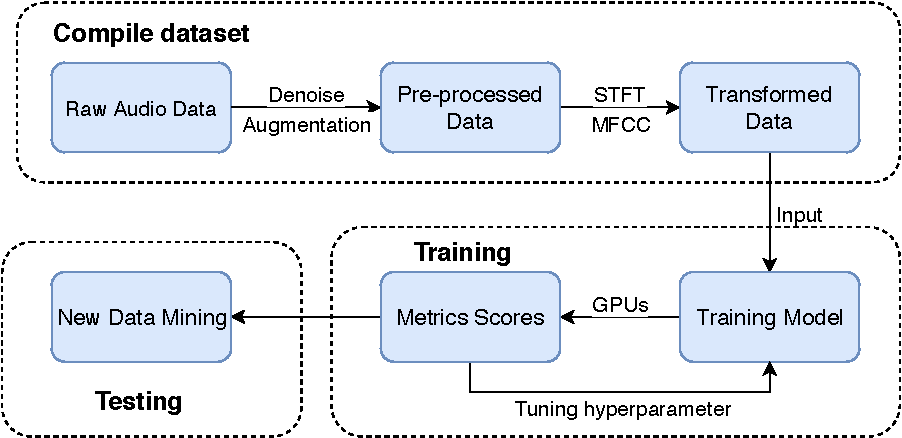
\includegraphics[scale=1]{Figs/intro/pipline.pdf}
  \caption{General steps of deep learning on audio data}
  \label{Fig:pipline}
\end{figure}
Audio as one of the data types has been developed as well. Via transforming time-series audio data into spectrograms, CNN can be applied to learn audio data based on spectral analysis. Fig.\ref{Fig:pipline} depicts the general steps of audio data detection in deep learning. There are three main procedures in audio data learning. First, the raw audio data need to apply signal processing methods for several purposes like denoising, clipping and augmentation. Afterwards, the time-series data are transformed into spectrograms as the input of CNNs model. Short-Time Fourier Transform (STFT) and Mel-Frequency Cepstral Coefficients (MFCC) are effective feature extraction techniques, transforming temporal characteristics into the spectral domain. During model training, different metrics are used to evaluate the performance, which is significant in tuning hyperparameters. If the model is fine-tuned, we can mine new data with significant accuracy. 

\section{Data Collection}
In this project, the audio data were recorded of endangered tropical primate Geoffroy's spider monkey, \textit {Ateles geoffroyi}. This species is significantly suitable for analysis since they highly depend on vocalized communication. With large contributions of Miss. Jenna Lawson who is a PhD student researching in Life Sciences, the raw audio data were labelled in an appropriate way. The spider monkey calls were collected by AudioMoth recording devices at a 48 kHz sampling rate, installed on the Osa Peninsula. This device generates minute-long files in \text{'.wav'} format and named by a hexadecimal code which represents the recording date and time. \par
In details with explanation by Jenna, there are 360 audio locations, each recording for 7 days, totals 36,800 hours of acoustic data over 2520 days of recording. Fig~\ref{fig:locations} demonstrates the habitat types and levels of protection audio data were found in, including 3 national parks, a reserve and unprotected regions on the Osa Peninsula of Costa Rica. It took one year to collect all the data and an additional 3 months of pilot studies to ensure that the spider monkeys actually make enough sounds to work and to test out the audio equipment. However, it is the most challenging effort to find the calls from the pilot data. Due to the rarity of spider monkey, only 388 presences of call were marked in 900 hours data, resulting in a small training dataset. Moreover, it took 30 more hours to record the positions in to 'Praat file'. Hence, the automated detection system is significantly necessary.

\begin{figure}[htp]
\centering
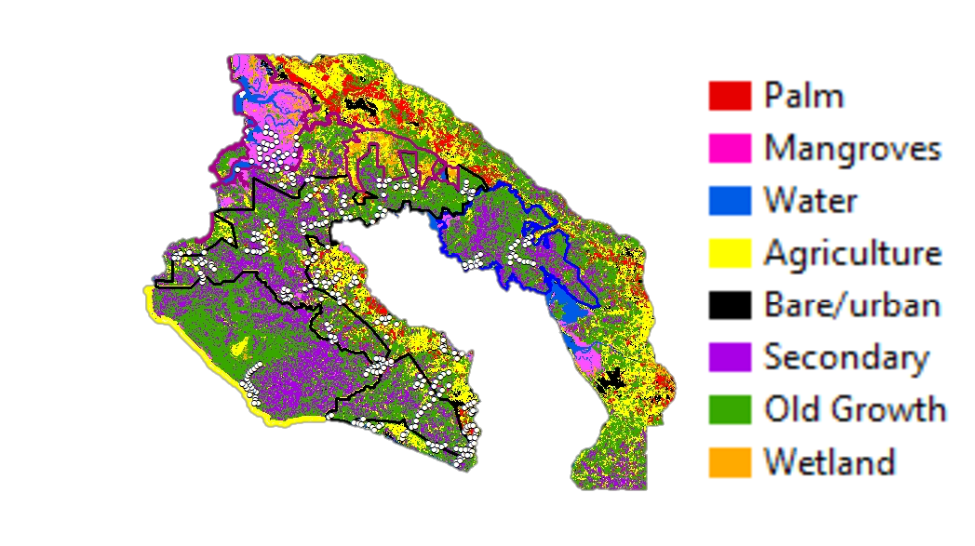
\includegraphics[scale=0.8]{Figs/intro/locations.pdf}
\caption{Locations of Osa Peninsula in Costa Rica (provided by Jenna)}
\label{fig:locations}
\end{figure}

\section{Aims and Organisation}
As a case study, this project is purposed to design and improve an automated detection system based on Deep Learning. The objectives are shown below:
\begin{itemize}
\item Pre-process the raw audio data into appropriate segments in order to extract the features effectively. Depending on mel-spectrogram of frequencies varying with time, compile the training and testing data. We aim to apply augmentation and denoising algorithms to evaluate performance.
\item Use self-designed CNN model to train the data as a baseline in a balanced way. Other applied methods of hard-negative-mining, weighted loss in the unbalanced dataset, denoising, and augmentation are as comparisons to evaluate model performance.
\item Use state-of-art like VggNet architectures with same train audio data. If the model is fine-tuning, then the model performance can have large improvement.
\item Use the trained model to predict new test acoustic data. Record and write the model predictions in files for manual check.
\end{itemize}
And the report is divided into six chapters and will be organized as follows:
\begin{itemize}
\item In Chapter 2, a background and literature review of audio data learning will be presented with parts of feature extraction and several studies of deep learning applied on audio data.
\item In Chapter 3, the methodology of pre-processing methods and basic theory of CNN will be introduced, including feature extraction, layers, the learning process of CNN, denoising and augmentation. The reasons for the chosen layers and loss function will be explained.
\item Chapter 4 will describe the implementation of this project and discuss the performance with evaluated metrics.
\item In Chapter 5 and 6, a summary will be presented of this project, following with the inspirations of future works.
\end{itemize}


% !TEX root=../main.tex
\chapter{Background}
\renewcommand{\baselinestretch}{\mystretch}
%\setlength{\parindent}{0pt}
\PARstart{T}{his} chapter is a summary of previous research based on audio data. Three main aspects of work were focused on where the performance has been improved. Firstly, different feature extract methods based on audio data are compared in previous studies. Two classical representation will be introduced, namely STFT and MFCCs. Afterwards, statistical learning and deep neuronal network models applied to audio data mining are compared in Section 2.2. Finally, studies of data pre-processing methods including noise reduction and augmentation are discussed. 
\section{Audio Feature Extraction}
When Welch~\cite{welch1967use} proposed a fast Fourier transform algorithm, namely short-time Fourier transform (STFT), efficient estimation of power spectra could be used on record analysis. He suggested segmental processing of the whole record and moving the window with possible overlapping, which can not only modify periodogram by averaging but also reduce computational complexity. Afterwards, Davis and Mermelstein~\cite{davis1980comparison} introduced Mel-frequency cepstral coefficients (MFCC) based on STFT. Due to the linear characteristic of Fourier transform, MFCCs are perceptual features which mimic received signal by the cochlea, aiming to enhance signal with significant contribution in phonetic detection. They firstly applied triangular mel-filters to scale spectrogram, then taking logarithm and discrete cosine transform (DCT) to calculate significant cepstral coefficients. \par
Lippends et al.~\cite{lippens2004comparison} compared performances of an auditory model and MFCC features in music genre classification task. They extracted 4 features from STFT and first 5 Mel-frequency cepstral coefficients classified by Gaussian Mixture Model (GMM), which shows that the auditory model has no outstanding accuracy than standard MFCC. Moreover, 12 identified MFCCs are used on recognition of anuran species~\cite{bedoya2014automatic}, achieving average accuracy in 99.61\% of all six species. However, MFCCs are not robust for the noisy environment, resulting in utilizing mel-spectrogram as representations. Choi et al.~\cite{choi2016automatic} compared STFT, MFCC and Mel-spectrogram (with accuracy 84.6\%, 86.2\% and 89.4\% respectively) using four layers of fully convolutional neural networks (FCN) on automatic tagging MagnaTagATune dataset. Similar work was studied in~\cite{huzaifah2017comparison} with additional fast
wavelet transform (FWT) and continuous wavelet transform
(CWT) as comparisons. He proved that mel-spectrogram still achieved significant performance on UrbanSound8K dataset among variations of settings, although STFT and CWT had some outstanding results on some models.\par
MFCC and mel-spectrogram are broadly used on automated species detection as well. Clemin et al.~\cite{clemins2003application} studied in recognizing African elephants sound based on GMM in 2003, resulting accuracies of 83.8\% for call and 88.1\% for identification.
Feature comparison of log-magnitude spectrogram using CNN and log-mel band energy using CRNN were studied in \cite{cakir2017convolutional}, improving the accuracy in 3\%. They stated that log-mel band energy makes bird sound more distinguishable. Another application on insect sound recognition was studied by~\cite{le2011insect}, using Probabilistic Neural Network (PNN) based on Bayesian classifiers. Although the identification accuracy is over 92\%, the method of selecting noise-free sections still introduced limitations in generalisation.

In summary, approaches of feature extraction significantly determine the performance of audio detection problems. By transforming time-series into cepstrum coefficients or spectrogram, the feature dimensions are reduced to a large extent. MFCCs present distinction on compressive representations which uses 12-20 coefficients as features~\cite{lippens2004comparison,le2011insect,clemins2003application}. Hence, it is beneficial to the linear statistical model, such as hidden Markov models and Gaussian Mixture Model. Mel-spectrogram is still an alternative with the advantage of noisy robustness. Therefore, mel-spectrogram is a suitable representation for deep learning, containing more distinguishable features.
\section{Automated Recognition Models}
In the past decade, hidden Markov models (HMM) and Gaussian Mixture model (GMM) were based on mathematical statistics. HMM aims to use observable data to predict the hidden feature based on the Markov process, for example predict event label with giving time-series signal. The property of the Markov process is that hidden variables of current time $s(t)$ only depends on previous time $s(t-1)$. Therefore, this property determined the suitability of speech recognition~\cite{rabiner1989tutorial} whose signals have relevance among context. Research based on HMM in antbirds recognition was studied by Vlad et al.~\cite{trifa2008automated}, who used optional MFCC features including energy, delta coefficients, acceleration. They found that varying estimated states from 5 to 15 could degrade performance dropped from 94.6\% to 82.5\%.\par
GMM is another general model since most of data in real life are subject to Gaussian distribution. Thus, using GMM by setting several mixtures can estimate the data distribution. Data can be considered as same label if they have a similar distribution. Brown \& Smaragdis~\cite{brown2009hidden} compared both GMM and HMM model on marine call types classification. The results proved that both these statistical models are powerful for acoustic classification of killer whales.
Zhao~\cite{zhao2017automated} used a sophisticated method of modelling log-band energy in order to automatically segment activities. The GMM-based model with two mixtures can capture both high-energy frames and low-energy frames, selecting the cross point as the threshold. Therefore, discriminative features of bird were selected, resulting in improved robustness of SVM to classify.

Both HMM and GMM are based on expectation maximum algorithm to estimate the probability of unknown parameters. Nevertheless, HMM takes temporal context into account, whereas GMM treats the whole signal as a unique spectral individual~\cite{brown2009hidden}. Comparing studies in~\cite{clemins2003application,trifa2008automated,zhao2017automated}, MFCCs were often used as features of GMM and HMM model. The reason may be that MFCCs largely compress the feature representations which make the statistical model easy to train. However, the mel-spectrogram can be consider as an effective alternative when using powerful models like CNN.

In recent years, deep learning has been rapidly developed on audio recognition since it can learn more effective features from input. Since VGGNet has outstanding performance on Large Vocabulary Continuous Speech Recognition (LVCSR)~\cite{sercu2016very}, convolutional neural network successfully applied on Acoustic Event Detection (AED) 80.3\% with accuracy~\cite{takahashi2016deep}. 
Moreover, Cakir et al.~\cite{cakir2017convolutional} proposed that using converlutional recurrent neural network (CRNN) with log-mel band energy as features improved the accuracy up to 88.5\% on bird event detection. Continue to bird detection, Grill et al.~\cite{8081512} designed two types of CNN architectures to detect the presence of bird call. General architecture designed with each convolutional layer following a pooling layer and using three dense layers, while local architecture used convolutional layers instead of dense layer transforming into a one-dimensional sequence and selected the maximum. Table \ref{tabel:summarymodel} makes a summary of these researches with different models and feature extraction methods. The types of recognition tasks and overall accuracy are recorded as well.
\begin{table}[htp]
\centering
\caption{Summary of models and feature extraction methods on species detection}
\label{tabel:summarymodel}
\begin{tabular}{ccccc}
\hline
Model& Species& Task& Feature& Accuracy(\%)\\
\hline
GMM& Elephant (2003)& Detection&MFCC& 83.8~\cite{clemins2003application}\\
HMM& Antbird (2008)& Detection&MFCC& 94.6~\cite{trifa2008automated}\\
GMM+HMM& Whales (2009)&Classification& MFCC & 92~\cite{brown2009hidden}\\
GMM+SVM& Bird (2017)& Classification& MFCC& $>$ 90~\cite{zhao2017automated}\\
PNN& Insect (2011)& Identification& MFCC& 92.44~\cite{le2011insect}\\
CNN& Bird (2017)&Detection& Log-spectrogram& 85.5~\cite{cakir2017convolutional}\\
CRNN& Bird (2017)& Detection& Log-mel energy
& 88.5 \cite{cakir2017convolutional}\\
CNN& Bat (2018)& Detection& STFT
& 89.6 \cite{batdetect18}\\
\hline
\end{tabular}
\end{table}
\section{Processing on Audio data}
For obtaining higher performance for species detection, several data processing method can be applied in order to improve the feature representation instead of inputting raw data. There are two main method that significant improve the performance of CNN model, specifically noise reduction and data augmentation. Noise reduction can enhance the region of interests (ROIs), making the call more distinct. Augmentation can increase the variation for training if only small number of data can be collected.

Generally, the acoustic recording is unavoidably introduced disturbance by the high-level noise, which related to the habitats that recording devices installed. Thus, environmental sounds have significant effects on the estimation of species' activity, introducing detection bias. As the denoising method implemented in~\cite{aide2013real,batdetect18}, regions of interests were enhanced with reducing the noise level. They applied spectral subtraction method which removed the mean amplitude in each frequency band as shown in \ref{fig:batnoise}. The level of background noise was suppressed to a large extent and removing the additive noise. Thus, the CNN model can effectively classify the foreground echo and the background noise with a high output probability of the presence of call. 
\begin{figure}[htp]
\centering
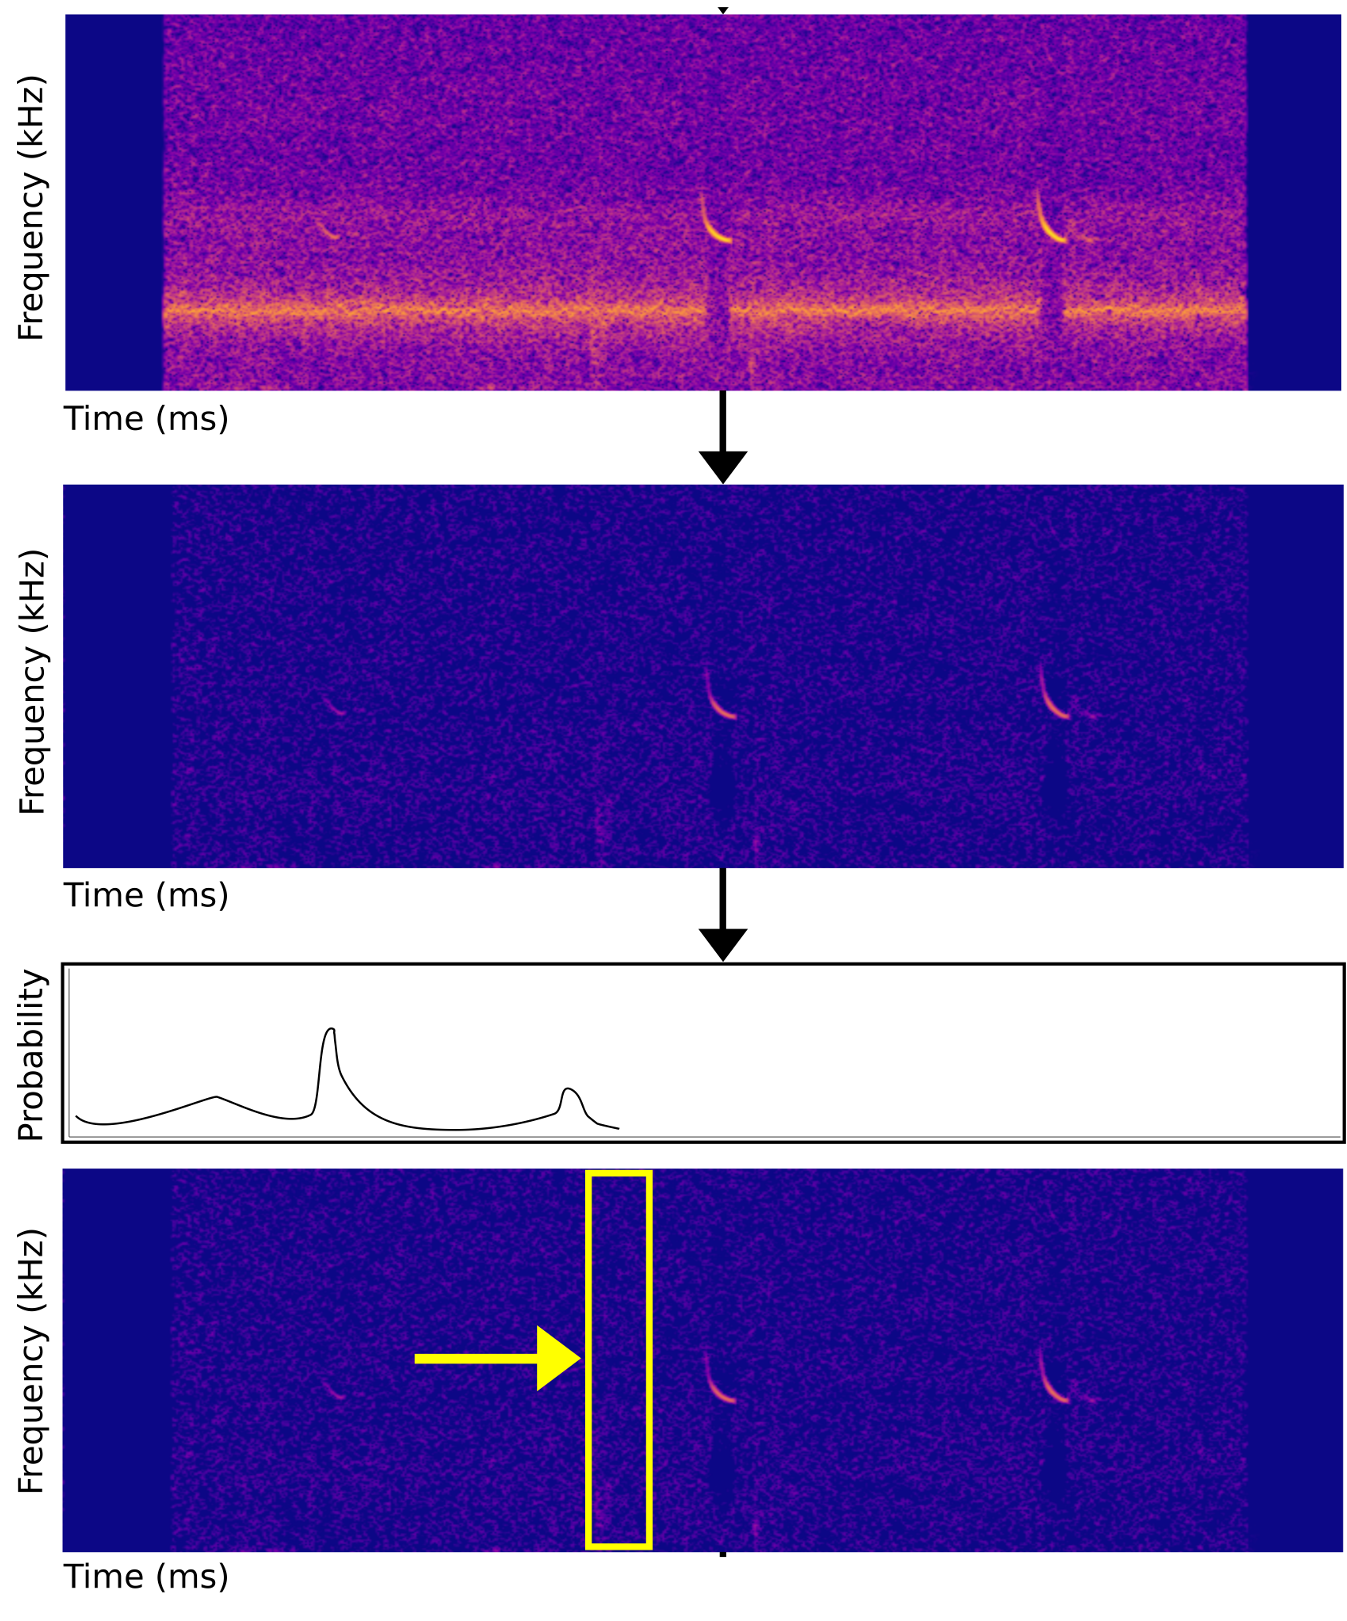
\includegraphics[scale=0.8]{Figs/chap2/batnoise.png}
\caption[Noise reduction of bat call]{Noise reduction of bat call in spectrogram representation~\cite{batdetect18}}
\label{fig:batnoise}
\end{figure}

Minimum mean-square error log-spectral amplitude (MMSE-LSA) estimator is another effective algorithm, which has been extensively implemented in automatic speech recognition (ASR) systems. Kim \& Rose~\cite{kim2002cepstrum} proposed a way of combining model based on MMSE-LSA to decompose noise and speech signal in the cepstral domain. Via combining MMSE-LSA technique with HMM model, the robustness of MFCCs is significantly increased. The MMSE-LSA estimator highly depends on a prior signal to noise ratio (SNR), which is estimated in the presence of non-speech region. Hence, \textit{a prior} SNR estimator based on CNN is introduced by \cite{nicolson2019deep}. The experiments by using deep learning showed the quality and intelligibility scores are much better than masking and mapping methods. However, there are fewer studies applied the MMSE-LSA for species detection tasks. In this project, I applied MMSE-LSA on 'whinny' calls to evaluate the performance.

Augmenting data is a necessary approach for model training especially on a small dataset. Takahashi et al.~\cite{takahashi2016deep} introduced a new augmentation method for audio event classification since the number of audio in each class is small. It is called Equalized Mixture Data Augmentation (EMDA) which mixes two different audio segments in the same class to synthesize new data. Moreover, he further modified the frequency characteristics by enhancing or disturbing a particular frequency band. By using augmentation, the accuracy was improved in 10\% compared with the original dataset. Other augmentation methods are compared in \cite{sprengel2016audio} as well for bird sounds identification, namely adding white noise, pitch shift, time shift and combining same class. He proved that time-shift took a large impact on performance, resulting in accuracy decreasing 3\% without applying time-shift. 



% !TEX root=../main.tex
\chapter{Methodology}
\renewcommand{\baselinestretch}{\mystretch}
\label{chap:method}
% \setlength{\parindent}{0pt}
\PARstart{T}{his} chapter will introduce the methodology of this project into two main aspects. One is to present pre-processing methods of audio data, including mel-spectrogram feature extraction, denoising method and data augmentation. The second aspect will introduce the architecture of CNN about activation function and different CNN layers. As to training CNN, the loss function and optimizer will be explained in the last section. 

\section{Mel-spectrogram Feature}
Spectrograms provide visual representations for people that can analyse the properties of audio data. As presented in Section 2.2, mel-spectrogram is an effective alternative for CNN as the input feature. However, the mel-spectrogram is based on the STFT which processed on discrete Fourier transform (DFT). It is expressed as $X_k=\sum ^{N-1}_{n=0}x_ne^{i2\pi \frac{kn}{N}}$, where $N$ coefficients are considered to represent the frequency value $X_k$. However, only several parts of audio we are interested since calls present a few seconds in most case. Therefore, separating the whole signal into shorter sections allows us to analyse the properties of particular points in time. By applying the window function to each segment, the STFT of signal can be obtained, which is expressed as
\begin{equation}
STFT\{ x_n\}(h,k)=X(h,k)=\sum_{n=0}^{N-1}x_{n+h}w_ne^{i2\pi \frac{kn}{N}}
\end{equation} 
where the length of window $h$ should be smaller than $N$. However, the represents of power spectrogram are non-uniform. Therefore, it is tough to extract informative features. By applying logarithm to power spectrogram can make representations more visual which is beneficial to analysis. Fig \ref{fig:powerlog} shows the difference of power spectrogram and spectrogram in the logarithm of example file '5AEF815A.wav'. Features are enhanced by taking the logarithm of the power spectrogram.\par 
\begin{figure}[htp]
     \begin{subfigure}[b]{0.5\linewidth}
         \centering
		  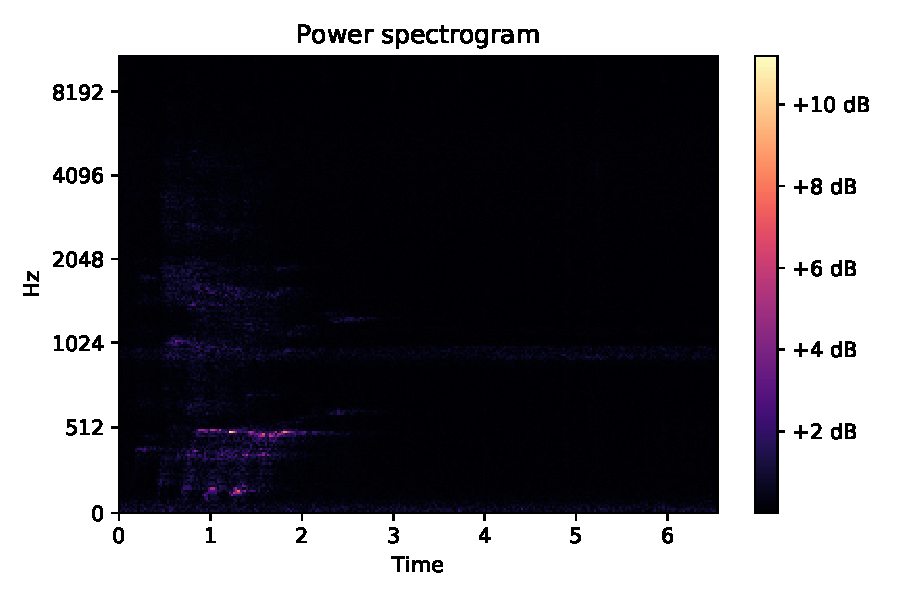
\includegraphics[scale=0.5]{Figs/chap3/power.pdf}
		  \caption{Power spectrogram}
     \end{subfigure}
     ~
     \begin{subfigure}[b]{0.5\linewidth}
         \centering
		  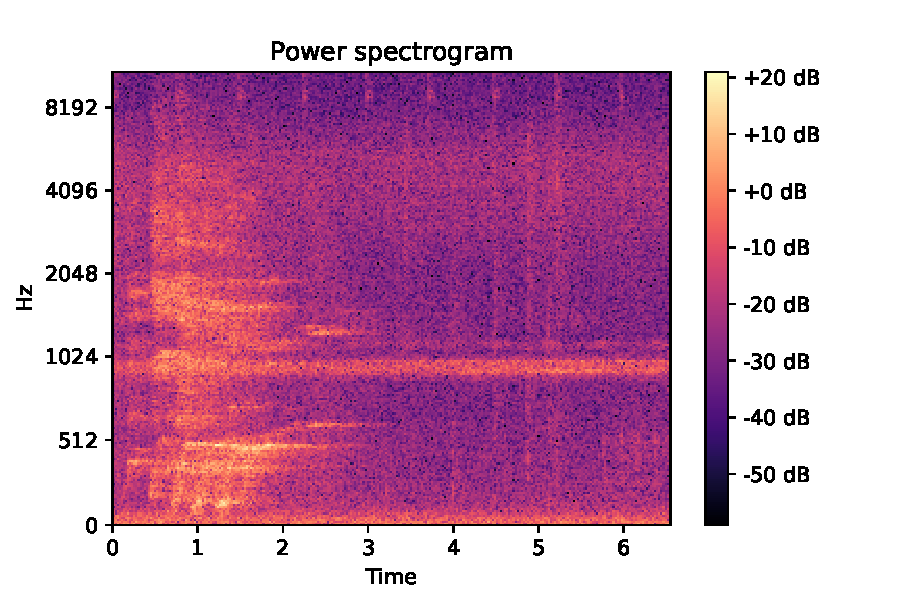
\includegraphics[scale=0.5]{Figs/chap3/logpower.pdf}
		  \caption{Log-scale spectrogram}
     \end{subfigure}
     \caption{Compare of power spectrogram and log-magnitude spectrogram (example file: 5AEF815A.wav)}
     \label{fig:powerlog}
\end{figure}
However, the STFT spectrogram is not the optimal extraction with the characteristic of linearity. By the inspiration of cochlea which can be considered as non-linear filters for the human sounds processing, the perceptual information can be introduced to the model. Specifically, emphasize the part of information which human listeners are sensitive and discriminative. After obtaining the short-time Fourier transform, the logarithm was applied to the magnitude to improve informative details. This process enhances the perceptual sensitive based on logarithmic-axis. Moreover, the frequency domain should be considered as well.

The mel-scale is one way to transform the original linear frequency into mel frequency. The mathematical approximation is 
\begin{align}
m&=2595\log_{10}(1+\frac {f}{700})\\
inverse: f&=700(10^{\frac{m}{2595}-1})
\end{align}
Therefore, the corresponding linear frequencies $f_i$ have equal perceptual distance by taking equally spaced mel-frequencies $m_i$. Fig~\ref{fig:melscale} (a) depicts the relationship between linear frequency in horizontal axis and the mel-frequency in vertical. However, other information will be degraded when using specific frequency $f_k$ during sampling the log-spectrogram. In other word, the transformation of mel-scale can be realized by applying filter bank to integrate the energy closed to the sample frequency $f_k$. 
\begin{equation}
u_k = \sum_{h=f_{k-1}+1}^{f_{k+1}-1} w_{k,h} |x_h|^2
\end{equation}
where $u_k$ is integrated energy in mel-spectrogram, $w_{k,h}$ is the weighted scalars and $x_h$ is the parts which close to sample frequency $f_k$. For the mel-scale, the weighted scalars are generally triangular function as shown in Fig~\ref{fig:melscale} (b). By combining weighted functions in non-linear spacing with 50\% overlapping, the log-spectrogram can be integrated and weighted.\par
\begin{figure}[htp]
     \begin{subfigure}[b]{0.5\linewidth}
         \centering
		  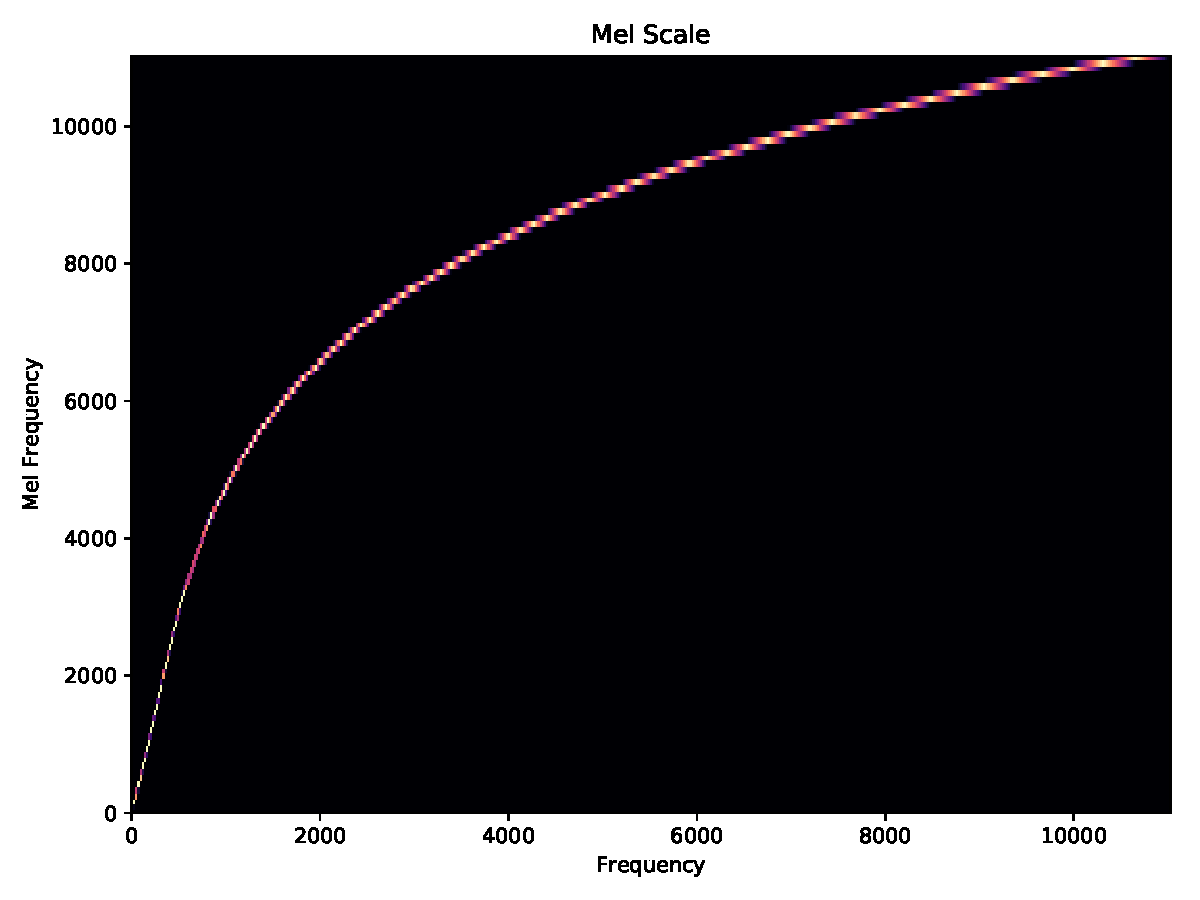
\includegraphics[scale=0.35]{Figs/chap3/mel_scale.pdf}
		  \caption{Mel scale function}
     \end{subfigure}
     ~
     \begin{subfigure}[b]{0.5\linewidth}
         \centering
		  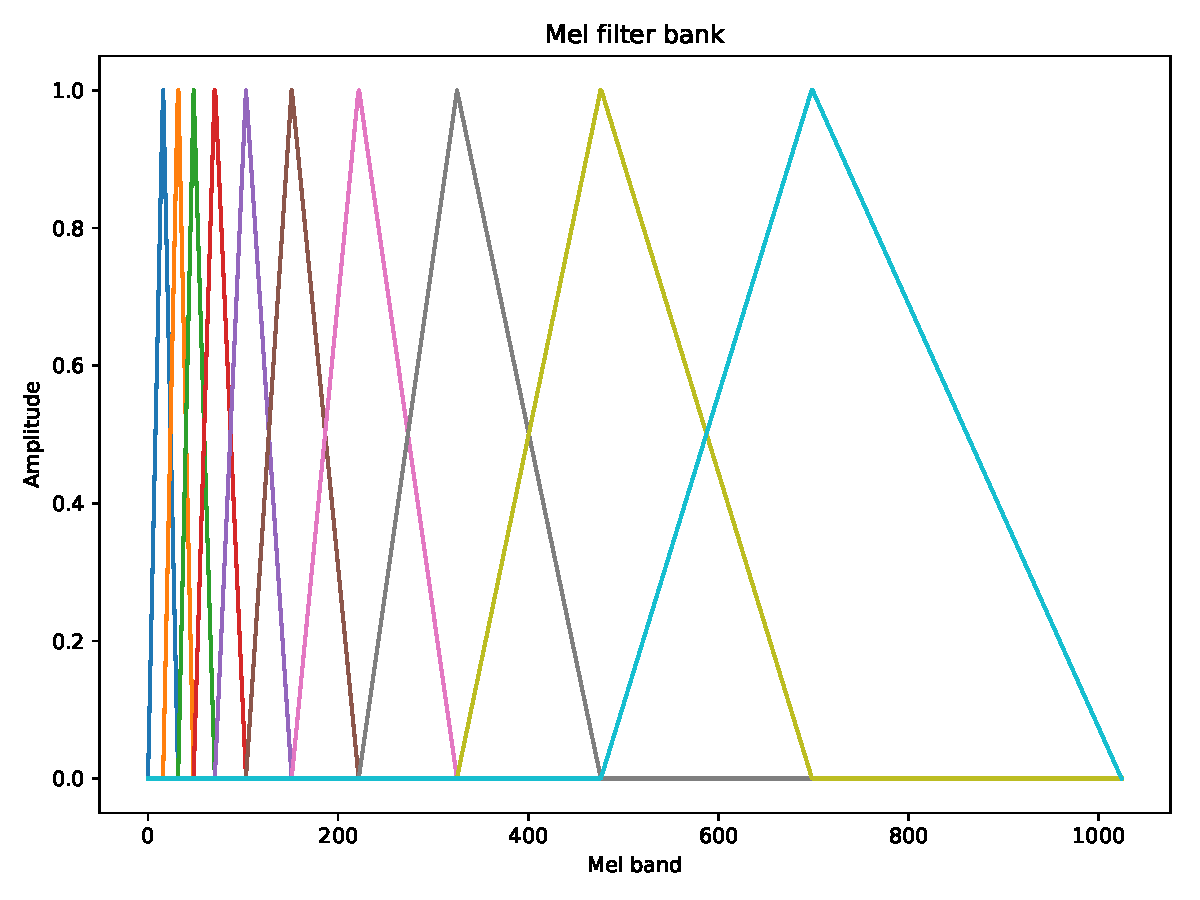
\includegraphics[scale=0.35]{Figs/chap3/mel_bank.pdf}
		  \caption{Mel filter bank with 10 mels}
     \end{subfigure}
     \caption{Transformation of frequency-to-mel and mel filter banks}
     \label{fig:melscale}
\end{figure}
By using triangular window above, the mel-spectrogram is obtained as show below. The mel-spectrogram contains more perceptual information which makes the presence of call more obvious. Therefore, using the mel-spectrogram as CNN model input can significant simulate how human make decisions. In addition, the MFCC can be calculated by taking discrete cosine transform (DCT) on log-scale mel-spectrogram. Due to MFCCs are not robust to additive noise, we chose mel-spectrogram as input feature.
\begin{figure}[htp]
\centering
  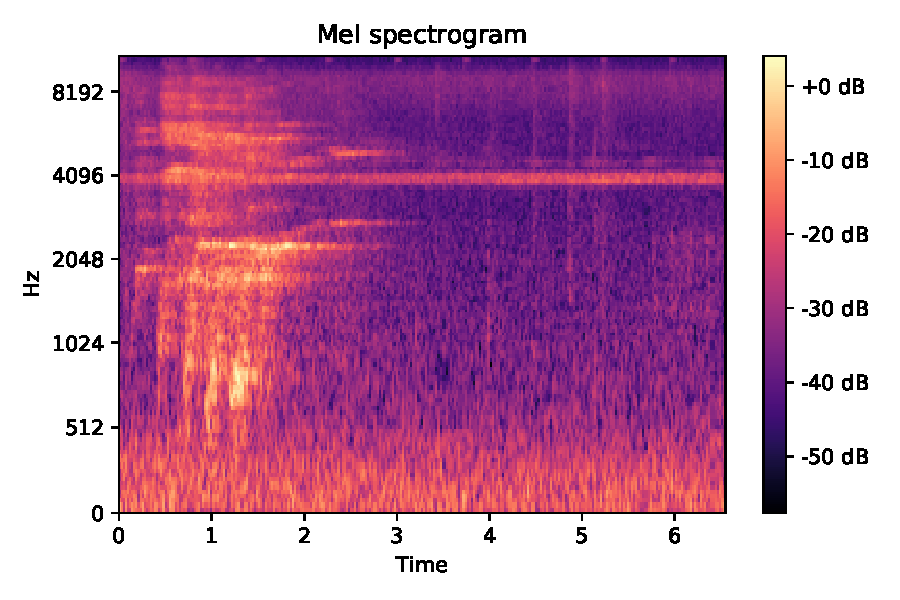
\includegraphics[scale=0.7]{Figs/chap3/mel_spec.pdf}
  \caption{Mel spectrogram}
 \label{fig:mel_spec}
\end{figure}
\section{Denoising Method}
The acoustic data of this project were recorded in the rainforest which caused complex and capricious environment. Thus, the signals of call presence were covered by large additive noise, resulting in inferior quality of audio. It is essential to apply denoising method to improve the signal noise ratio (SNR). We compared two performance of common denoising method, namely spectral subtraction~\cite{boll1979suppression} and MMSE-LSA estimator~\cite{ephraim1985speech}. First of all, as stated in their study, assume of the received noisy signal is 
\begin{equation}
y(t)=x(t)+n(t)
\end{equation}
where $x(t)$ is the desired signal and $n(t)$ is the noise. Thus, the equation above in frequency domain represents as
\begin{align}
Y(\omega)&=X(\omega))+N(\omega)\label{eq:spectrum}
\\
\notag
\end{align}
Only $y(t)$ and $Y(\omega)$ are known values. The objective of the denoising method is to reduce the noise interference without influencing the quality of the informative signal.
\subsection{Spectral Subtraction}
The aim of spectral subtraction is to estimate the power of noise based on the frequency domain $\hat N(\omega)$. Afterwards, the estimated spectrum of desired signal $\hat X(\omega)$ is obtained by
\begin{equation}
\hat X(\omega)=Y(\omega))- \hat N(\omega)
\label{sub-spec}
\end{equation}
Since the additive noise has the flat power along with the whole frequency band, the noise spectrum $\hat N(\omega)$ can be estimated as the expectation of noise spectrum $E\{|N(\omega)| \}$. This can be calculated by averaging parts where only noise recording presents at that time. The estimated noise spectrum can be denoted as 
\begin{equation}
\hat N(\omega)=E\{|N(\omega)| \}\cong |\bar N(\omega)|= \frac{1}{K}\sum_{i=0}^{K-1} |\bar N_i(\omega)|
\end{equation}
where $|\bar N_i(\omega)|$ is the i-th amplitude of K frames of noise. Therefore, the desired signal in frequency domain is calculated by the equation~\ref{sub-spec}. Hence, the time-series signal $x(t)$ is the inverse-Fourier transform of $\hat X(\omega)$.\par
The spectral subtraction estimator is a primary and effective method of noise reduction. The algorithm for estimating the noise spectrum is simple, resulting in less computing complexity. However, this approach assumes that the additive noise is wide-band and stationary, which does not always correspond to reality. Therefore, the reconstructed signal has a deviation to the theoretical desired signal in most cases. A large disturbance will be introduced due to the significant variations between estimated noise and actual noise As a consequence, the contributive information is distorted by the disturbance.
\par
Observing the original noisy mel-spectrogram in Fig~\ref{fig:mel_spec}, the presence of call is concentrated on the area of 512$\sim$3000 Hz frequency bands. It is notable that the uniform noise appears at 4096 Hz all the time. Fig~\ref{fig:spec_sub} demonstrates the  mel-spectrogram of reconstructed signal after using spectral subtraction estimator. Although the background was suppressed to a large extent, the estimator affects the quality of desired information as well. 
\subsection{MMSE Log-Spectral Amplitude Estimator}
As expressed in Eq~\ref{eq:spectrum}, the Fourier transform of noisy signal $Y(\omega)$, desired signal $X(\omega)$ and noise signal $N(\omega)$ can be expressed in complex form, which consists of amplitude spectral and phase spectral. Thus, for the $k$th frequency bin, the observed signal is expressed below:
\begin{align}
Y(\omega_k)&=X(\omega_k)+N(\omega_k)\\
R_k\exp(j\theta_k)&=A_k\exp(j\alpha_k)+N_k
\end{align}
where $R_k$, $A_k$ and $N_k$ are corresponding amplitude spectrums. Due to the noise is assumed as additive white Gaussian noise (AWGN), there is no phase spectrum of noise, resulting in . Hence, if we estimate the amplitude of desired signal $A_k$, the restored signal can be reconstructed by using phase of received signal.
\par
The MMSE-LSA estimator is an improved noise reduction method based on the MMSE short-time spectral amplitude~\cite{ephraim1985speech}. It has large difference of spectral subtraction which estimates the noise spectrum based on average frames. Nevertheless, the objective of MMSE-LSA is to minimise the mean-squared error between the actual log-amplitude of speech signal and log-amplitude of estimated signal, which can be expressed as 
\begin{align}
\arg\min_{\hat{A}_k}{\mathbb{E}\left[\left(\log A_k-\log\hat{A}_k\right)^2\vert y(t),0\leq t\leq T\right]}
\end{align} 
given the known condition of observed signal $\{ y(t), 0\leq t\leq T\}$. Obviously, the optimal solution for this problem is when the estimated amplitude equal to actual amplitude, leading to zero MMSE error. That is,
\begin{equation}
\hat A_k=\text{exp}\left\{\mathbb{E}\left[\ln A_k | Y_k\right]\right\}
\end{equation}
Based on the Gaussian model assumption, the term $\mathbb{E}\left[\ln A_k | Y_k\right]$ is calculated given by $Y_k$. Let $Z_k=\ln A_k$ and the moment function $\Phi_{Z_k|Y_k}(\mu)$ is
\begin{align}
	\Phi_{Z_k|Y_k}(\mu)&=\mathbb{E}\left\{\text{exp}(\mu Z_k) | Y_k\right\} \notag\\
	&= \mathbb{E}\left\{A_k^\mu | Y_k\right\} \label{eq:aa}
\end{align}
Thus, the aim is to calculate $\Phi_{Z_k|Y_k}(\mu)$ now and obtain $\mathbb{E}\left[\ln A_k | Y_k\right]$ by taking derivative of moment function at $\mu=0$. The moment function can be obtained from equation \ref{eq:aa}:
\begin{align}
\Phi_{Z_k|Y_k}(\mu)&=\mathbb{E}\left[A_k^\mu\vert Y_k\right] \\
&=\int_0^{\infty}\int_0^{2\pi}a_k^\mu p(a_k,\alpha_k\vert Y_k)d\alpha_k d a_k \\
&= \int_0^{\infty}\int_0^{2\pi}a_k^\mu \frac{p(a_k,\alpha_k,Y_k)}{p(Y_k)}d\alpha_k d a_k \\
&=\frac{ \int_0^{\infty}\int_0^{2\pi}a_k^\mu p(Y_k\vert a_k,\alpha_k) p(a_k,\alpha_k) d\alpha_k d a_k }{ \int_0^{\infty}\int_0^{2\pi} p(Y_k\vert a_k,\alpha_k) p(a_k,\alpha_k) d\alpha_k d a_k }
\end{align}
Since we assumed that each frequency bin confirms to Gaussian distribution, the probability was defined as following:
\begin{align}
p(Y_k\vert a_k,\alpha_k)&=\frac{1}{\pi\lambda_d (k)}\exp\left[ -\frac{1}{\lambda_d (k)}\vert Y_k - a_k e^{j\alpha_k} \vert^2 \right] \\
p(a_k,\alpha_k&)=\frac{1}{\pi\lambda_x (k)}\exp\left[-\frac{a_k^2}{\lambda_x (k)}\right]
\end{align}
where $\lambda_x (k)\triangleq \mathbb{E}\left[\vert X_k \vert ^2\right]=A_k^2 $ and $\lambda_d (k)\triangleq\mathbb{E}\left[\vert D_k \vert ^2\right]$. 
Based on the deduction in \cite{ephraim1985speech}, the amplitude of pure speech signal is calculated by
\begin{align}
\hat{A}_k=\frac{\xi_k}{1+\xi_k}\exp\left[\frac{1}{2}\int_{\upsilon_k}^{\infty}\frac{e^{-t}}{t}dt\right]R_k
\label{eq:magni}
\end{align}
and following parameters need to be estimated
\begin{align}
\upsilon_k\triangleq \frac{\xi_k}{1+\xi_k}\gamma_k;\quad
\xi_k\triangleq\frac{\lambda_x (k)}{\lambda_d (k)};\quad
\gamma_k\triangleq\frac{R_k^2}{\lambda_d (k)}
\label{eq:snr}
\end{align}
$\xi_k$ and $\gamma_k$ are considered as \textit{a prior} and \textit{a posterior} SNR respectively. The variance of noise can be updated by the voice activity detection (VAD) to detect the section without the presence of speech. Afterwards, \textit{a prior} SNR can be obtained by decision-directed method. Algorithm \ref{alg:mmse} demonstrates the procedure of MMSE-LSA estimator in Python realisation.\par
\begin{algorithm}
	\renewcommand{\algorithmicrequire}{\textbf{Input:}}
	\renewcommand{\algorithmicensure}{\textbf{Output:}}
	\caption{MMSE-LSA estimator for Python realisation}
	\label{alg:mmse}
	\begin{algorithmic}[1]
		\REQUIRE Noisy signal $y(t)$
		\ENSURE Enhanced signal $x(t)$
		\STATE Calculate the number of frames $N$ based on sampling frequency $f_s$
		\STATE Assume first 6 frames is noise/silence
		\FOR {k $\rightarrow$ 6}
		\STATE Windowing $y(t)$ in frame length $y(k)$
		\STATE FFT: y(k) $\rightarrow$ $Y(\omega_k)$
		\STATE Calculate variance of noise power $\lambda_d(k)$
		\ENDFOR 
		\FORALL{frames $k$ in $N$}
		\STATE FFT: y(k) $\rightarrow$ $Y(\omega_k)$
		\STATE Compute the power of noisy signal $R_k^2$
		\STATE Compute and limit a post SNR to avoid overflows $\gamma_k<40 dB$
		\STATE Calculate a priori SNR $\xi_k$ based on previous magnitude as shown in Eq.\ref{eq:snr}
		\STATE Estimate the magnitude of clean signal $X_k$ based on Eq.\ref{eq:magni}
		\ENDFOR
		\STATE IFFT: $X(\omega)\rightarrow x(t)$
		\STATE \textbf{return} $x(t)$
	\end{algorithmic}  
\end{algorithm}
Fig \ref{fig:logmmse} shows the mel-spectrogram after applying the MMSE-LSA estimator. Comparing with Fig \ref{fig:mel_spec}, the noise level was reduced to a large extent, presenting in lower magnitude of background. Moreover, the magnitude of call was enhanced, instead of attenuating in Fig \ref{fig:spec_sub}. Thus, the performance for MMSE-LSA method is outstanding than spectral subtraction in theoretically.
\begin{figure}[!htp]
     \begin{subfigure}[b]{0.5\linewidth}
         \centering
		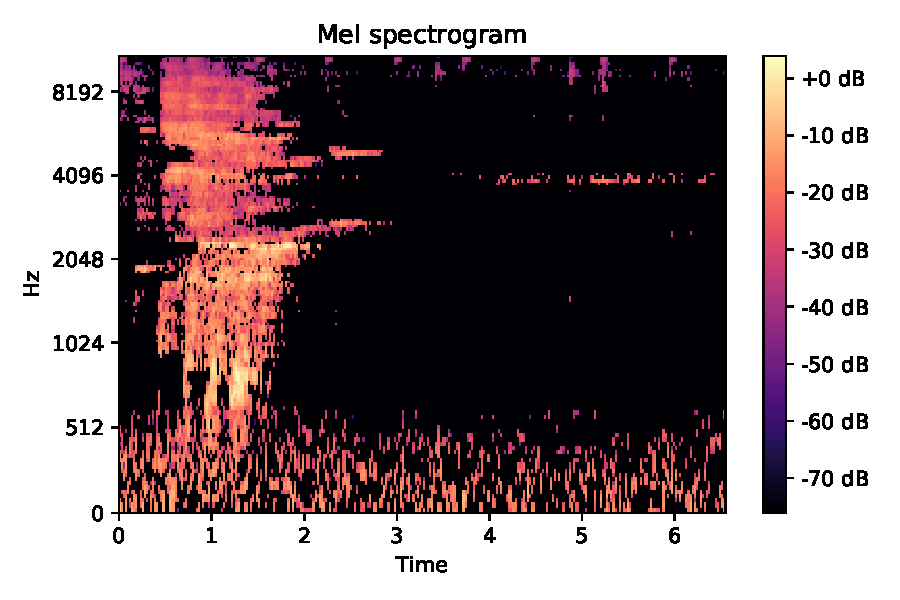
\includegraphics[scale=0.5]{Figs/chap3/sub_spec.pdf}
		\caption{spectral subtraction}
		\label{fig:spec_sub}
     \end{subfigure}
     ~
     \begin{subfigure}[b]{0.5\linewidth}
         \centering
		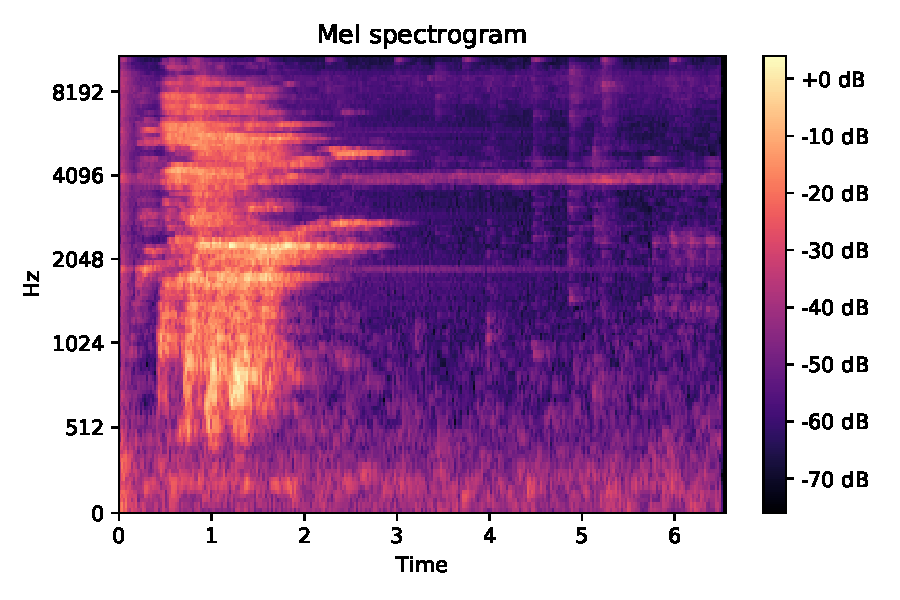
\includegraphics[scale=0.5]{Figs/chap3/logmmse.pdf}
		\caption{MMSE-LSA}
		\label{fig:logmmse}
     \end{subfigure}
  \caption{Mel spectrogram by using noise reduction methods}
  \label{Fig:denoise}
\end{figure}
\section{Data Augmentation}
For a CNN model, millions of weighted parameters need to be trained in hidden layers, which needs a mass of data to ensure the network fully trained. As to this project, since only 388 calls were collected for training, the data have to augment, avoiding the over-fitting problem. Moreover, it can improve the variation and generalisation of the model. I applied five common and effective augmentation methods to artificially generate data both on positives and negatives as similarly done by \cite{sprengel2016audio}. In addition, all augmentation methods are implemented in the time domain. For each augmentation, I randomly selected one of them to manipulate.
\begin{itemize}[leftmargin=*]
\item \textbf{Time-shift}\\
The audio signal is shifted in time with random position. Representing in the spectral domain is equivalent to vertically splinted the spectrogram into two segments. Time-shift will change the order of these two parts, resulting in sharp changes at joint. However, the model task is to detect the presence of whinny call which has less semantic relations among context. Furthermore, the total information is reserved. With this approach, the network has the ability to handle the irregular spectrogram and detect the call occurred at any time.
\item \textbf{Add noise}\\
Adding background noise is one of the most effective approaches to improve network performance. In section 3.2, I introduced the noise reduction method that enhances the speech region. However, the performance of model would pull down if only the denoised dataset was trained. At this circumstance, the model is biased with less generalisation, presenting in only recognizing noise-free clips. Hence, I added moderately amplitude of noise to the original file, combining with the noise reduced data to train. Moreover, I mixed part of negative samples to positive as well. 

\item\textbf{Pitch \& Speed}\\
As different augmentation methods were compared in \cite{schluter2015exploring}, the result showed that the pitch shift is significantly beneficial for improving. The pitch shift will change the frequency of sounds, resulting in vertical shift in the spectrogram. However, a large range of pitch shift will affect the biological features, which is not helpful for training. Time stretch will change the speed of the data. In order to maintain the same length of data, zeros were padded for speeding up and latter parts were removed for slow down mode. I applied a 5\% range of pitch shift and 10\% range of time stretch on raw data.
\item\textbf{Amplitude}\\
Changing amplitude is another way of augmentation. Since the version of data has large environmental noise, raising up the amplitude proved not a beneficial way. Hence, I emphasized to reduce dynamic amplitude with gain in $0.5\sim1.1$. 
\end{itemize}

\section{Design of CNN}
\subsection{Activation Functions}
In deep learning, the neuron is the basic unit which mimics the way of human brain transmitting and processing. The artificial neuron is a mathematical model that contains input, computing and output modules. With different connection ways between neurons, the neuronal network can realize a amount of tasks. As to a fully connection, each neuron will receive inputs from previous neurons and forward transmitting the processed result. This can be expressed in mathematical:
\begin{align}
\mathbf z^l &=\sigma(\mathbf w^l \mathbf a^{l-1}+b)
\end{align}
where $\mathbf w$ is the weight at current layer which need to be learned, $\mathbf a$ is the output of last layer, $\mathbf z$ is the neuron output, $\sigma$ is the activation function and $b$ is the scalar bias.

However, there is no activation function for perceptron model, whose final output is linear combinations of the input feature. This leads to a limited capability of network to deal with complex problem. Hence, the non-linearity activation functions are introduced so that the feature representation of DNN is powerful. By setting the number of neurons at each layer, the network can converge to arbitrary functions. Four common non-linear activation functions will be introduced as follows. In addition, Fig \ref{Fig:act} shows the output curves for each functions.
\begin{itemize}[leftmargin=*]
	\item \textbf{Sigmoid}\\
	The mathematical expression of sigmoid is denoted as
	\begin{equation}
		\sigma(x)=\frac{1}{1+e^{-x}}
	\end{equation}
	It is one of the non-linear activation functions. The advantage of sigmoid function that maps the infinite range value in limited range $(0, 1)$, which can be interpreted as the neuron firing rate. Thus, most of binary classification networks used sigmoid as the final output, indicating the positive or negative. However, two main shortcomings make sigmoid function less use in the hidden layer. Firstly, due to the nearly zero slope at large positive and negative regions, gradient vanishing problem appears at the process of back propagation, which makes network refuse to further learn. Moreover, the output of sigmoid is not zero-centred with all positive values. This causes the weight updating always in one direction (positive or negative). 
	\item \textbf{Tanh}\\
	As shown in Fig \ref{fig:sig}, the tanh function has the similarity of the sigmoid function, which can be expressed as
	\begin{equation}
		\tanh(x)=\frac{e^{x}-e^{-x}}{e^{x}+e^{-x}}=2*sigmoid(2x)-1
	\end{equation}
	Although the tanh solved the zero-centred problem of sigmoid, gradient vanishment is still an issue for tanh during back propagation.
	\item \textbf{ReLU \& eLU}\\
	ReLU is the short term of rectified linear unit and the expression is denoted as
	\begin{equation}
	A(x) = max(0,x)	
	\end{equation}
	Although it is simple in mathematics, many of studies prove the outstanding performance of ReLU \cite{maas2013rectifier}. Firstly, the computational cost is quite small (only need to judge the input if is positive). Therefore, it converges faster than tanh and sigmoid function. Additionally, it overcomes the gradient vanishing problem in the positive region. However, the output of ReLU is still not zero-centred. Due to forced rectifying to zero for negatives, the dead ReLU problem appears for some neurons which will never be activated. For solving this problem, leaky ReLU and eLU are introduced, changing the function in negative part.\\
	Exponential Linear Units, namely eLU, has all distinctions of ReLU. The negative part is modified into an exponential function, which is robust for noise. The average output of eLU is near zero without dead neuron problem. Thus, it should be outstanding compared with ReLU function, in spite of increasing computation. Nevertheless, few experiments demonstrated that the performance of eLU is better. Hence, I selected ReLU function applied in the design of CNN architecture.
\end{itemize}
\begin{figure}[!htp]
     \begin{subfigure}[b]{0.5\linewidth}
         \centering
		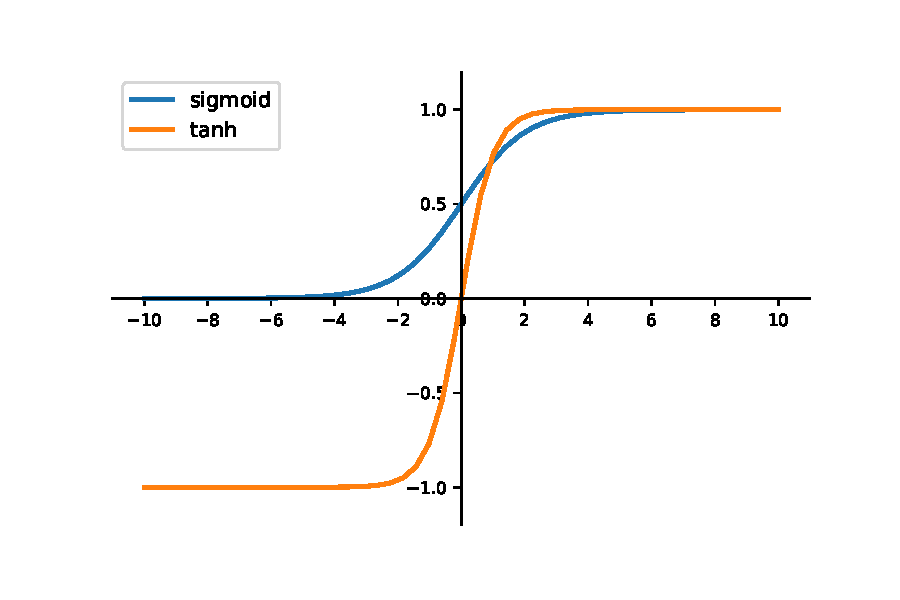
\includegraphics[scale=0.5]{Figs/chap3/act1.pdf}
		\caption{Sigmoid and tanh}
		\label{fig:sig}
     \end{subfigure}
     ~
     \begin{subfigure}[b]{0.5\linewidth}
         \centering
		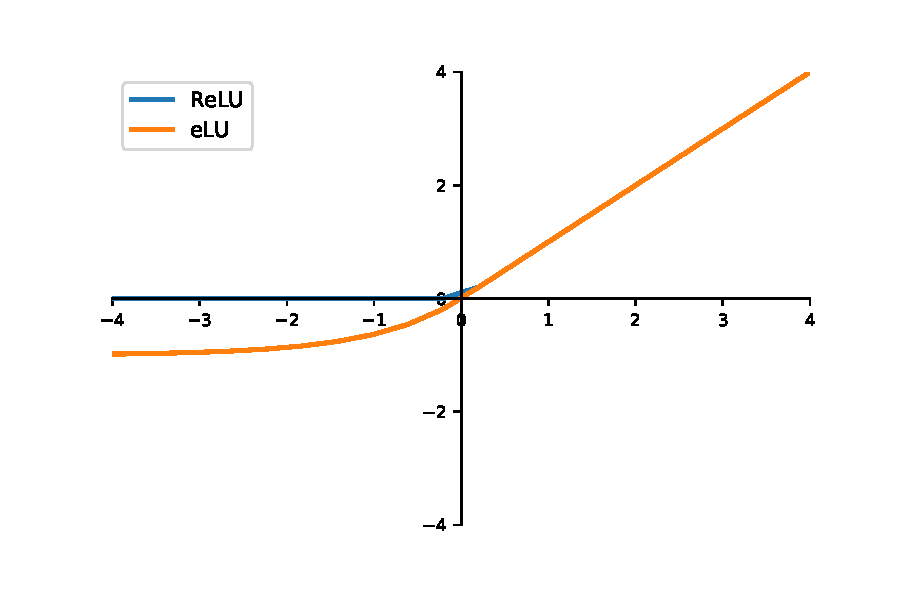
\includegraphics[scale=0.5]{Figs/chap3/act2.pdf}
		\caption{ReLU and eLU}
		\label{fig:relu}
     \end{subfigure}
  \caption{Different activation functions output curve}
  \label{Fig:act}
\end{figure}
\subsection{Layers of CNN}
The network is designed by a combination of different layers. In general, there are three main layers for CNN architecture, connecting in hierarchical order.
\begin{itemize}[leftmargin=*]
	\item\textbf{Convolutional layers}\\
	The convolutional layer is the principal layer of CNN, which is used to extract features. It is performed by applying certain size filters to the input, accumulating masked values to get one output. With different weights in filters, the output can learn diverse features. Fig \ref{fig:filter} depicts the operation of filter convolution. For example, applying a $5\times5$ filter to the input will obtain one individual output. However, $5\times5$ size filter can be replaced by using two successive $3\times3$ filters, resulting in the same shape of output. This is the basic operation of VGG Network which makes network deeper.
	\begin{figure}[htp]
	\centering
	  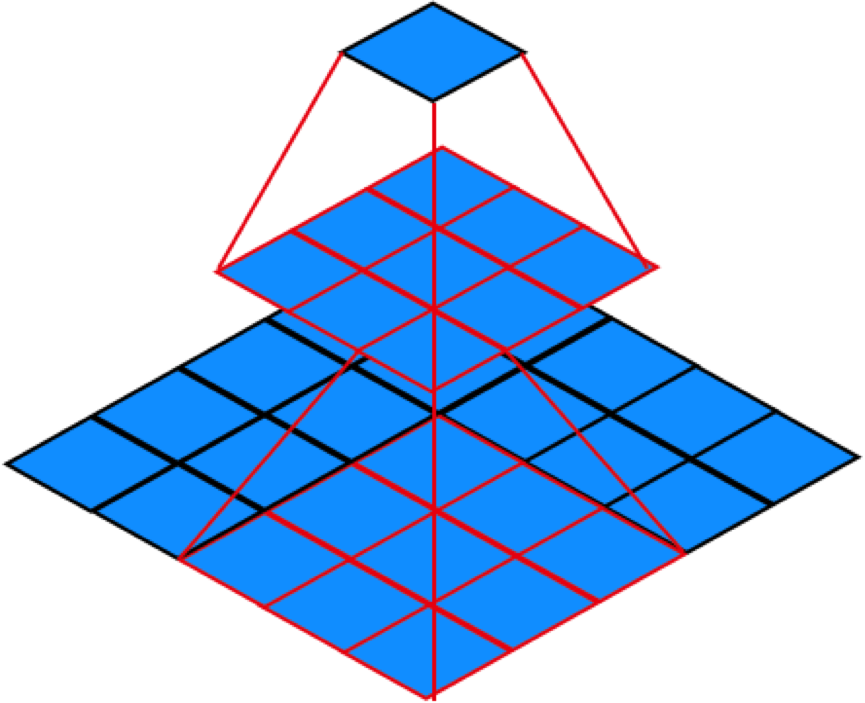
\includegraphics[scale=0.5]{Figs/chap3/vggfilter.png}
	  \caption{visualisation of convolutional filters in VGGNet}
	 \label{fig:filter}
	\end{figure}
	\item\textbf{Pooling layers}\\
	Pooling layers are normally following with convolutional layers. There are two aims of pooling that one is to reduce the dimension of parameters after convolution. On the other, the extracted features are compressed by selecting significant feature. In this project, maximum pooling layers were used to extract the maximum value in the corresponding region. It is an important procedure to prevent network over-fitting. Meanwhile, the computation speed is accelerated due to reducing feature dimension.
	\item\textbf{Fully-Connected (Dense) layers}\\
	Fully-connected or dense layers are the final section of the network. It firstly transforms the matrix into vector representation via convolving the matrix of each neuron. With FC layers, all neurons in current layer are connected to the next layer. Hence, features are combined in order to fit the distribution of data. Softmax or sigmoid activation functions are applied at the end as the classification output of the model.
\end{itemize}
\section{Model Training}
\subsection{Loss Functions and Optimizer}
Loss function plays an important role in training network and assists in back propagation. For a time step, the input data will pass through the CNN network and obtain a prediction at the end layer. A loss is generated to measure the divergence between the actual label $y$ and the prediction $\hat y$. As to one epoch, all training samples losses of each time step are summed together to calculate the back propagation step. The expression is 
\begin{equation}
\boldsymbol{\mathcal{L}}(\boldsymbol{\theta})=\frac{1}{n}\sum_{i=1}^{n}L\big(y^{(i)},f(\mathbf{x}^{(i)},\boldsymbol{\theta})\big)
\end{equation}
where $\mathbf{x}$ and $\boldsymbol{\theta}$ are training samples and learning features respectively, $f(\cdot)$ represents the model output. There are several different loss functions, dealing with various tasks. Cross entropy (CE) is one of extensively used function with outstanding performance, especially in classification problem \cite{simard2003best}. In our case, the learning problem is a binary classification task which needs model to detect the positives and negatives. Hence, binary cross-entropy was applied for this work. The mathematical expression is shown below,
\begin{equation}
\boldsymbol{\mathcal{L}}=-\frac{1}{n}\sum_{i=1}^{n}\big[y^{(i)}\log(\hat{y}^{(i)})+(1-y^{(i)})\log(1-\hat{y}^{(i)})\big]
\label{eq:loss}
\end{equation}
The former term measures the positive prediction loss and the latter is for negative. Thus, if the true label is positive/negative (1/0) while the prediction is far different from the actual label, a large loss is introduced. Due to only logarithm and summation operation, the gradient can be computed rapidly compared with MSE loss function. 

Once we defined the loss function, the optimiser needs to be chose for converging up to global optimum. An outstanding optimiser has the capability of not only fast convergence but also maintaining model recall. Adaptive moment estimation (Adam) optimiser \cite{kingma2014adam} computes both first and second-order moment to gradient descent. Since the mean and uncentered variance of the gradient are estimated, the Adam optimiser can adaptively adjust learning momentum, resulting in fast convergence speed compared with other gradient descent algorithms. As shown in practical experiments \cite{ruder2016overview}, Adam optimiser has an impressive performance. Thus, we apply Adam optimiser to reduce loss in Eq \ref{eq:loss} with default values of $\beta_1$, $\beta_2$ and $\epsilon$. The learning rate was set to $10^{-5}$. 
\subsection{Hyperparameter Tuning}
After constructing the network, the model needs to be trained with appropriate parameters. The metrics are significant for evaluating the performance of model, which concentrates on targets of true positives (TP), false positives (FP), true negatives (TN) and false negatives (FN). Based on these targets, four different metrics are used to evaluate the network, namely accuracy, precision, recall and F1 score. Accuracy is the general metric to assess the performance. Precision represents how many true positives were detected among positive predictions, which is the ratio of TP with the summation of TP and FP. Recall evaluates how many positives can be mined by model, which is TP/(TP+FN). F1 score is the weighted combination of recall and precision. Hence, the model can be considered as optimum whichever achieves the expressive accuracy and F1 score.

Even though we use the fixed dataset to train the model, the eventual objective is to reduce generalisation error as much as possible. Thus, tuning network is an important part of training. As to tuning hyperparameters, the validation dataset is applied to evaluate performance during model training. It differs from test dataset that when the model is fine-tuned, the validation set will add to the training set for the final training. By observing metrics of the validation set, the hyperparameters can be tuned. Due to the limited GPUs and the size of dataset, the batch size is set to 16. 
\begin{itemize}[leftmargin=*]
	\item \textbf{Training Epoch}\\
	For one time step, the CNN model will only concentrate on the batch size of data. When all training data are learned forward and updated backwards once, the CNN network is trained for one epoch. Thus, with large training epochs, the model could learn features multiple times. However, the model is insufficiently trained if epoch is too small. Hence, the threshold needs to be determined. By excessively set epoch to make model over-fitting on purpose, the appropriate threshold is easy obtained. Fig \ref{Fig:learning} demonstrates the training and validation loss with 100 epochs. After 50 epochs, the validation loss decreases significantly slowly compared with training loss. The difference between validation and training becomes larger, which caused the over-fitting problem on training data. Therefore, the epoch is set to 50.
	\begin{figure}[htp]
	\centering
	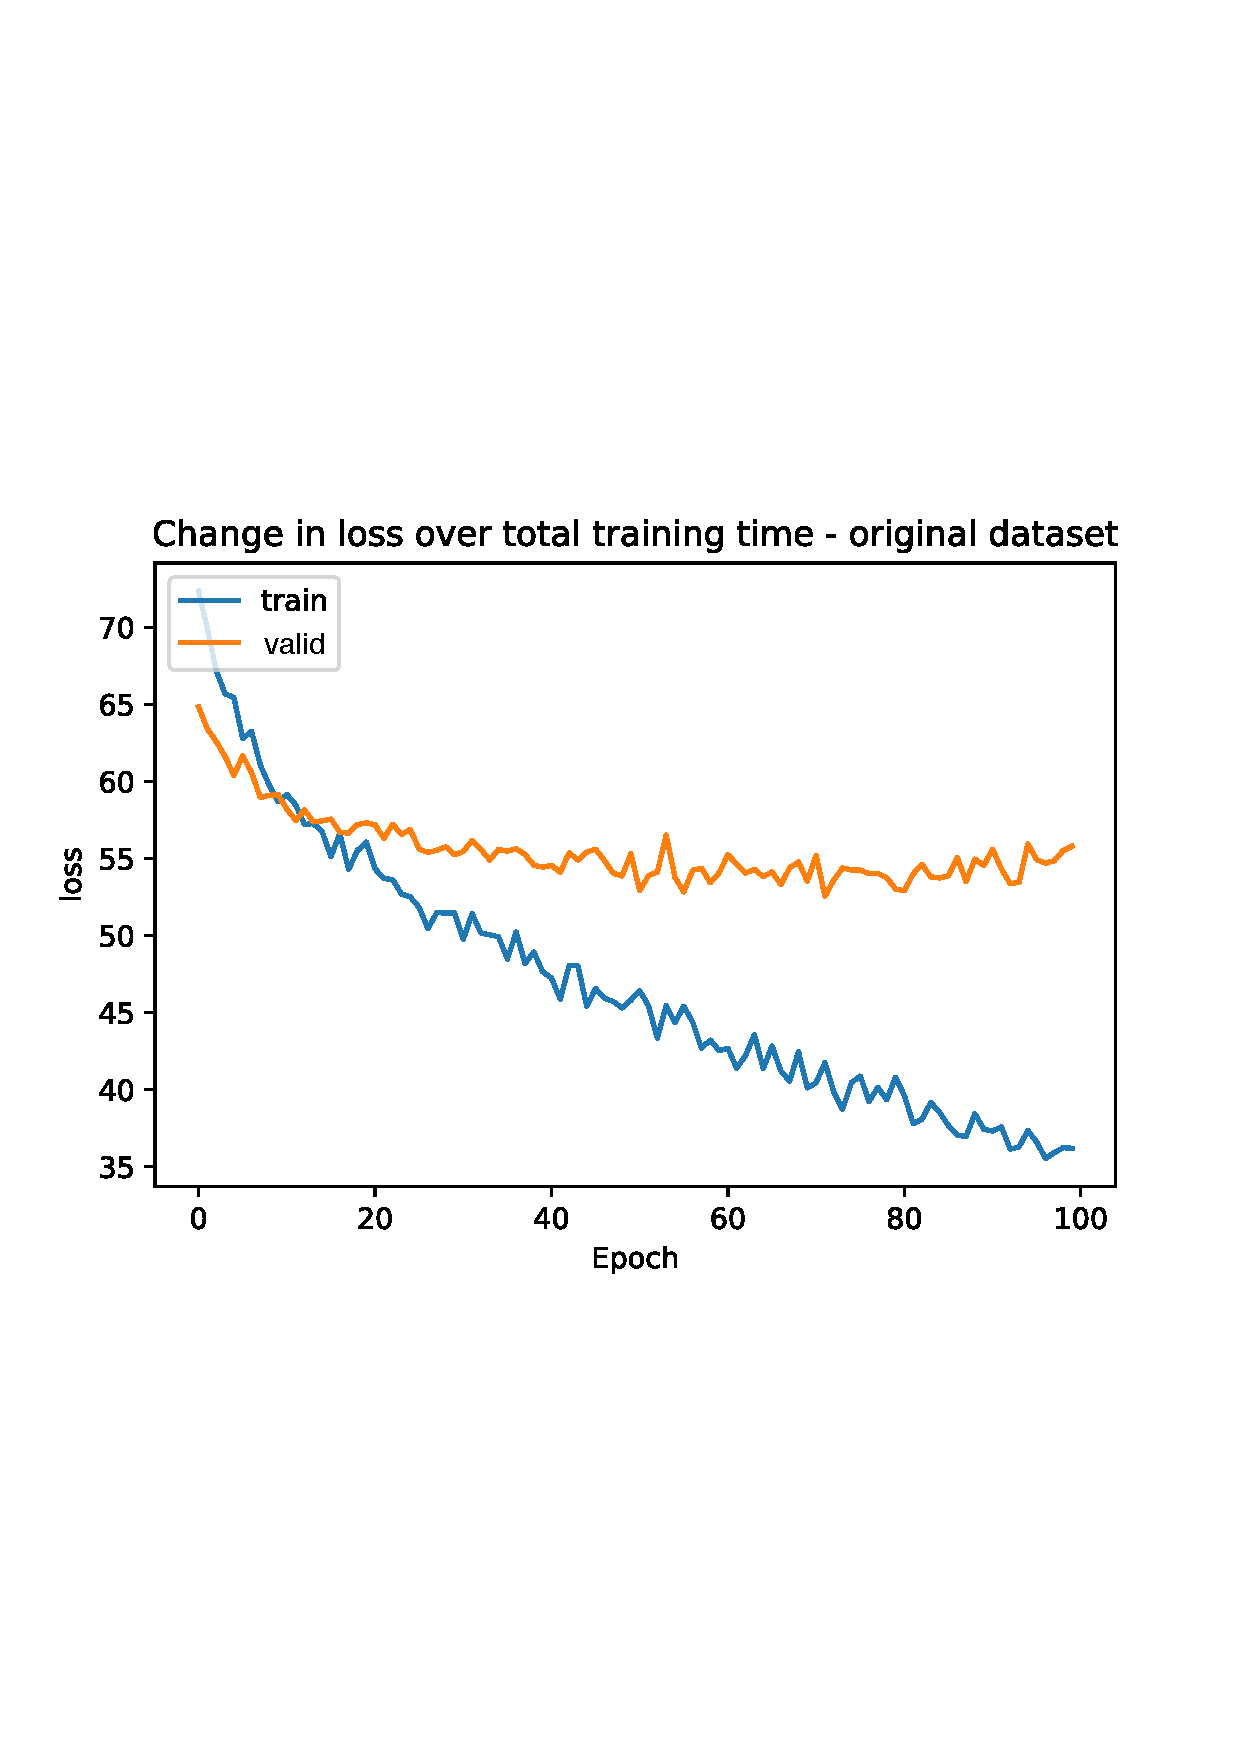
\includegraphics[scale=0.45]{Figs/chap3/e100.pdf}
	\caption{Training and validation loss curves of 100 training epochs}
	\label{fig:epoch}
	\end{figure}
	\item \textbf{Learning rate}\\
	Learning rate of the optimiser is another parameter that affects the loss. Although a large learning rate can rapidly converge to the optimum, it will result in the zigzag problem, oscillating near the global optimum. Fig \ref{Fig:learning} depicts the loss of learning rate in $10^{-4}$ and $10^{-5}$. The model appears over-fitting problem after 20 epochs in Fig \ref{fig:10-4}, presenting in an increasing trend of validation loss. When reducing learning rate 10 times, the loss slightly falling down without over-fitting. Thus, the learning rate is determined as $10^{-5}$, even if the final loss is large.  
	\begin{figure}[htp]
     \begin{subfigure}[b]{0.5\linewidth}
         \centering
		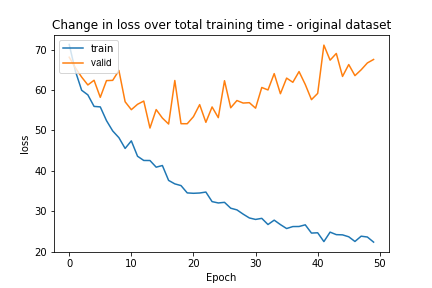
\includegraphics[scale=0.5]{Figs/chap3/10-4.png}
		\caption{learning rate=$10^{-4}$}
		\label{fig:10-4}
     \end{subfigure}
     ~
     \begin{subfigure}[b]{0.5\linewidth}
         \centering
		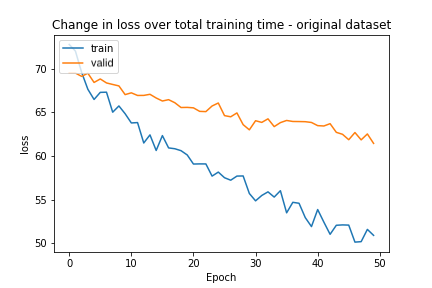
\includegraphics[scale=0.5]{Figs/chap3/10-5.png}
		\caption{learning rate=$10^{-5}$}
		\label{fig:10-5}
     \end{subfigure}
  \caption{Training and validation loss curves of varying learning rate}
  \label{Fig:learning}
\end{figure}
\end{itemize}

\subsection{Hard Negative Mining}
In this project, the negative data consists of other animal calls, environmental sounds and white noise. Since the negative examples are relatively effortless to obtain compared to rare positive calls, the number of negative examples is more than that of positives. Therefore, the variance and quality of negatives have large differences. For example, the white noise is significantly easy to be classified while other animal calls are not. As to further improving the model performance, hard negative mining approach can be applied to model training. Experiments proved this method is effective on objective detection tasks by SVM \cite{felzenszwalb2009object} and region-CNN (R-CNN) \cite{girshick2014rich}. They firstly used random bounding boxes to train the model. The boxes without overlapping with positives are called easy negatives and those with part of targets are difficult to be classified. Subsequently, these hard negatives were selected to form a new hard-negative dataset and retrain the model. After repeating several times, the performance of model is improved to a large extent. 
	\begin{figure}[!htp]
	\hskip-1.5em
     \begin{subfigure}[b]{0.5\linewidth}
         \centering
		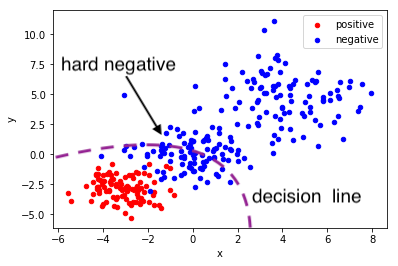
\includegraphics[scale=0.55]{Figs/chap3/pn.png}
		\caption{original data}
		\label{fig:pn}
     \end{subfigure}
     ~
     \begin{subfigure}[b]{0.5\linewidth}
         \centering
		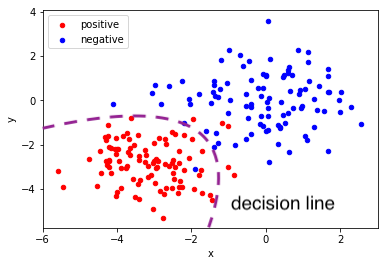
\includegraphics[scale=0.55]{Figs/chap3/hnm.png}
		\caption{hard negatives}
		\label{fig:hn}
     \end{subfigure}
  \caption{Hard negative mining examples in two-dimension}
  \label{Fig:hnm}
\end{figure}

Fig \ref{Fig:hnm} demonstrates the principle of hard negative mining in two-dimensional representation. The negatives with near distance to positives are hard samples to be classified. Thus, the decision boundary is influenced by the easy negatives for first trained.  A large amount of negatives are classified as positives. When applying hard negative mining method, only hard samples are selected for the second train. Thus, the decision boundary is more distinct compared with the first training model, resulting in outstanding accuracy. As to this work, the hard negative mining only applied once to train the model totally twice.


  
% !TEX root=../main.tex
\chapter{Implementation and Results}
\renewcommand{\baselinestretch}{\mystretch}
\label{chap:results}
% \setlength{\parindent}{0pt}
\PARstart{T}{his} chapter demonstrates the implementation steps based on the theory of previous section. Firstly, the acoustic data of Geoffroy’s spider monkey is clipped and extracted in order to compile the dataset. The baseline model was contributed by Duncan Bulter who studied this relevant project last year. The improvement methods are concentrated on audio denoising, augmentation and hard negative mining. Moreover, a complex deep learning model with the inspiration of VGGNet is proposed and tested. The generalisation error is measured by new test data clips for both models.

\section{Dataset Compiling and Feature Extraction}
\subsection{Data preparation}
The raw audio data are minute-long files in Waveform Audio File Format (WAVE). With the support of software 'Praat', accurate time locations about when the spider monkey call occurs in the minute-long files were recorded in files. However, the raw file is significantly redundant to apply audio data detection. Hence, all of raw files need to be clipped into appropriate length segments. By observing the length of segments of interest, the average length of calls is approximate 1 second and the longest call is 2.1 second. Thus, we selected 3-seconds window to be used for clipping minute-long files. Based on the Python library \texttt{pydub}, the audio file can be manipulated as time series in milliseconds. Firstly, the accurate start and end time of calls were read from Praat-files. Since the duration of calls is smaller than the window length, residual segments can be randomly chose to form 3-seconds clips, which can increase the variety of dataset. Moreover, for guaranteeing the quality of calls, a 20\% margin is restricted between the edge of the window and the edge of call duration. \par
By following these steps, totally 388 positives are clipped from raw data files, corresponding to the statement in Section 1.3. Crump \& Houlahan (2017)~\cite{crump2017designing} stated that the performance of recognizers can be improved by selecting files from different sites as the training dataset. As stated in Section 1.3, seven different locations of audio data are successively named by type 1 to 7. Table \ref{tabel:Positives} depicts that the type-1 \& 6 data occupy a higher percentage of the positive dataset where other types are as complementary.
\begin{table}[h]
\begin{center}
\caption{Number of Positive files in different types}
\label{tabel:Positives}
\begin{tabular}{ | c | c| c | } 
\hline
Type & Num. of Positives & Percentage of whole data (\%) \\ 
\hline
Type-1 (cattappa) & 126 & 32.47 \\ 
Type-2 (osa) & 18 & 4.64 \\ 
Type-3 (shady) & 38 & 9.79 \\ 
Type-4 (other) & 47 & 12.11 \\ 
Type-5 (live-recording) & 25 & 6.44 \\ 
Type-6 (will) & 77 & 22.38 \\ 
Type-7 (tape-recording) & 57 & 14.69 \\ 
\hline
\end{tabular}
\end{center} 
\end{table}\par
As to creating initial negative examples, two different strategies are used. These are:
\begin{itemize}
\item[(1)] randomly sampling from regions in minute-long files which do not contain the spider monkey call, mainly including additive Gaussian noise and environment sounds;
\item[(2)] collecting quantities of other animals' calls in relevant regions, such as howler monkeys, birds and macaws.
\end{itemize}
Additionally, all sampled negatives are 3-seconds length clips without containing the calls of interest. As a result, there are two types of initial negatives dataset that 450 negative files contain clipped environment sounds and noise and another 288 files of other animal calls. Hence, the total number of negatives are approximate twice of positives. As to constructing dataset, the number of negatives is balanced as same as positives. However, the initial negative training data contain a number of white noise called easy negative example, which is effortless for the CNN model to classify. Therefore, the balanced negatives set was firstly appending 288 other animal calls then randomly selecting the remaining number of negatives from noise dataset.
Moreover, the technique of hard-negative-mining was applied as similarly implemented by Mac Aodha et al.~\cite{batdetect18}. Two ways were used for searching for challenging negative examples. Firstly, the initial negative clips were considered as hard examples if they were incorrectly classified with scores over 0.5. Secondly, I successively clipped raw minute-long files into plenty of 3-seconds clips. Then, use the early-stage model to predict all clips and false positive clips are selected as hard examples. \par
\subsection{Data processing}
The original training dataset contains 776 examples with the half number of positives and negatives. The pre-processing methods introduced in Section 3.2 and 3.3 are compared with the original dataset without processing (w/o). These methods are processed based on the time-series signal. As a consequence, a new folder with the processed file were created. Afterwards, the network will be trained by using different files. The number of denoised fold is same as the dataset without processing. Three groups of data were tested, which are denoised method with spectral subsection (SS), the denoised method with MMSE-LSA and hard negative mining based on MMSE-LSA. As to the data augmentation method, I repeat augmented function 5 times to enlarge the number of dataset, resulting in 3880 files in total. For each augmentation, the strategy was random chose from five methods introduced in Section 3.3. Even if the strategies are selected same, the margin and amplitude are still randomly determined. Thus, the diversity and variety of data can be guaranteed.

Before feeding into the CNN network model, the audio data feature were extracted represented as mel-spectrogram. Due to the Python library \texttt{librosa}, the MFCC features were effectively extracted with sample rate of a 48 kHz, 50\% overlap and hamming filter with over 20 ms per frame, resulting in a window size of 1024 samples. Thus, the shape of spectrogram is (128, 282). For evaluating model, the whole dataset was separated into the training set and test set at a ratio of 9:1. 

\section{Baseline Model}
\subsection{Architecture}
Based on the previous work of Duncan, we chose his designed model as the baseline as shown in Fig \ref{fig:baseline}. He defined a CNN model with three convolutional layers with one size $28\times5\times5$ and two $48\times5\times5$. The filter moves one stride without zero paddings. With the activation function of 'Relu', following by MaxPooling layers with size $4\times2$. He added batch normalization layer only after the second convolution layer. Afterwards, flatten layer was applied with 6048 features and feeding into a dense layer with 128 neurons. The prediction score was the output of the sigmoid function in the region of 0$\sim$1. The input and output shapes after each layer are demonstrated in the Appendix \ref{Fig:shapebaseline}. Due to the binary classification problem, the loss function was binary cross-entropy. Moreover, the Adam optimizer with a fixed learning rate $10^{-5}$ was chosen to upgrade weights. Since there are 698 training data, the model was trained in 50 epochs with batch size 16. \par
\begin{figure}[htp]
\centering
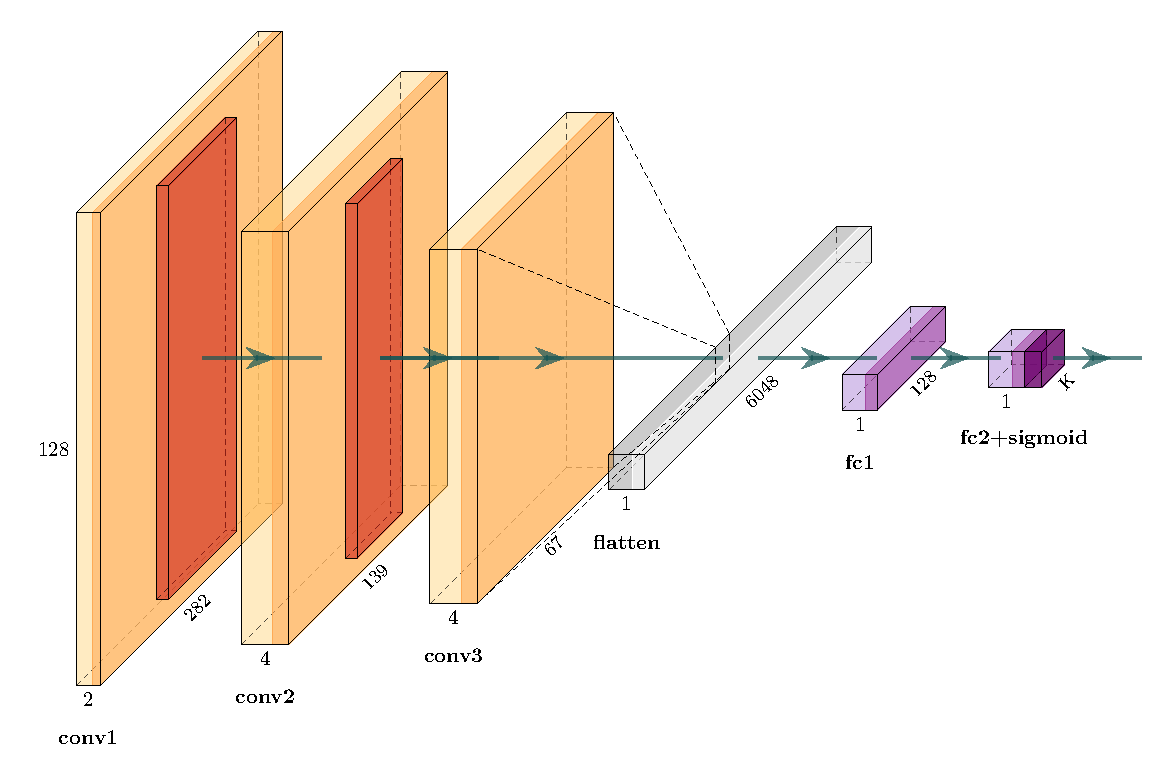
\includegraphics[scale=0.55]{Figs/chap4/baseline.pdf}
\caption{Architecture of the baseline CNN}
\label{fig:baseline}
\end{figure}
Therefore, the baseline model is a relatively shallow convolutional network compared with VGG16 and ResNet. It learns low-level feature to classify the example, which may restrict the performance on detection. The model was first trained with the initial negative training dataset. Then, applied hard negative mining method to train the second time.
\subsection{Results}
\subsection*{Normalization \& Balanced}
The baseline model was separately trained to demonstrate the effects of balanced and normalised data. The strategy of the balanced dataset is introduced in Section 4.1.1 and the number of unbalanced dataset consists of 388 positives calls and 738 negatives. The normalisation was applied both on time-series signal before extraction and on the logarithmic magnitude mel-spectrogram. Table \ref{tab:balanc} shows the metrics scores of these strategies.\par
\begin{table}[htp]
    \centering
    \caption{Scores of balanced and unbalanced dataset with/without normalization}
    \label{tab:balanc}
    \resizebox{0.9\textwidth}{!} & 60.87 & 60.26  & 65.38  & \textbf{66.99}   \\ \hline
    \textbf{Precision\%}      & 57.84                & 52.04      & 65.32    & \textbf{67.75}      \\ \hline
    \textbf{Recall\%}   & 66.18        & 54.89        & \textbf{67.07}      & 63.13   \\ \hline
    \textbf{F1\%}          & 61.43                     & 50.10    & \textbf{66.1}     & 64.89     \\ \hline
    \end{tabular}}
\end{table}
For the dataset without normalisation, the balanced data has a relatively low precision, which means that plenty of negatives are classified as false positive. The unbalanced dataset fails to improve the performance without normalisation, presenting in nearly 50\% precision, recall and F1 score. As to the normalised dataset, both balanced and unbalanced dataset obtain over 60\% scores. The balanced one attains enhanced recall and F1 score, while the accuracy and precision of unbalanced model are a little better.

Normalisation is a significant part before training. Due to the audio data were collected in the volatile tropical environment at different locations, the within-class variance for both positives and negatives are significantly large. Hence, without normalisation, the model will be disturbed by the non-uniform data distribution during training. As shown in Table \ref{tab:balanc}, the accuracy and F1 score are improved 5\% for the balanced dataset. The precision has significant improved and slightly increase in recall since all data were normalized to the range $0\sim1$. As to unbalanced dataset, normalisation can reduce the diversity of data distribution to a large extent, presenting in a distinct increment of all metric scores. Therefore, the unbalanced normalised dataset achieves the highlighted accuracy and precision. However, the recall and F1 scores still fall down. In general, training with unbalanced dataset seems less helpful for performance. The reason may be that, due to the unbalanced number of data, the model tends to concentrate more on negatives, which causes the decline of recall and F1 score. As a result, training with normalised unbalanced dataset achieves a relatively higher accuracy and precision with 66.99\% and 67.75\% respectively. Recall and F1 score are outstanding of the balanced normalised dataset. Observing metric scores in overall, the normalised balanced data strategy was determined to be used.

\subsection*{Pre-processed methods}
As to evaluating the data processing methods, three groups of results are shown in Table \ref{tabel:base  dataset} as control groups on performance. In order to control variables, all dataset are balanced and normalised before training, as discussed in previous section. It took nearly 40 minutes to train the model with 698 data and more than 1.5 hours for augmentation on CPU.
\begin{table}[htp]
\centering
\caption{Metrics scores of baseline model with data processing methods}
\label{tabel:base dataset}
\resizebox{0.9\textwidth}{!} & \textbf{Precision\%} & \textbf{Recall\%} & \textbf{F1 score\%} \\ \hline
\textbf{Orig: Initial} & 65.38 & 65.32 & 67.07 & 66.1 \\
\textbf{Orig: hnm} & 69.23 & 82.34 & 61.65 & 69.85 \\ \hline
\textbf{SS: Initial} & 73.08 & 76.17 & 58.89 & 65.86 \\
\textbf{LSA: Initial} & 76.92 & \textbf{84.10} & \textbf{75.72} & \textbf{78.79} \\
\textbf{LSA: hnm} & 74.36 & 82.05 & 68.72 & 73.41 \\ \hline
\textbf{Aug: Initial} & 76.29 & 78.27 & 71.72 & 73.53 \\
\textbf{Aug: hnm} & \textbf{77.84} & 83.72 & 68.89 & 74.54 \\ \hline
\end{tabular}}
\end{table}
\begin{figure}[!htb]
     \begin{subfigure}[b]{0.5\linewidth}
         \centering
          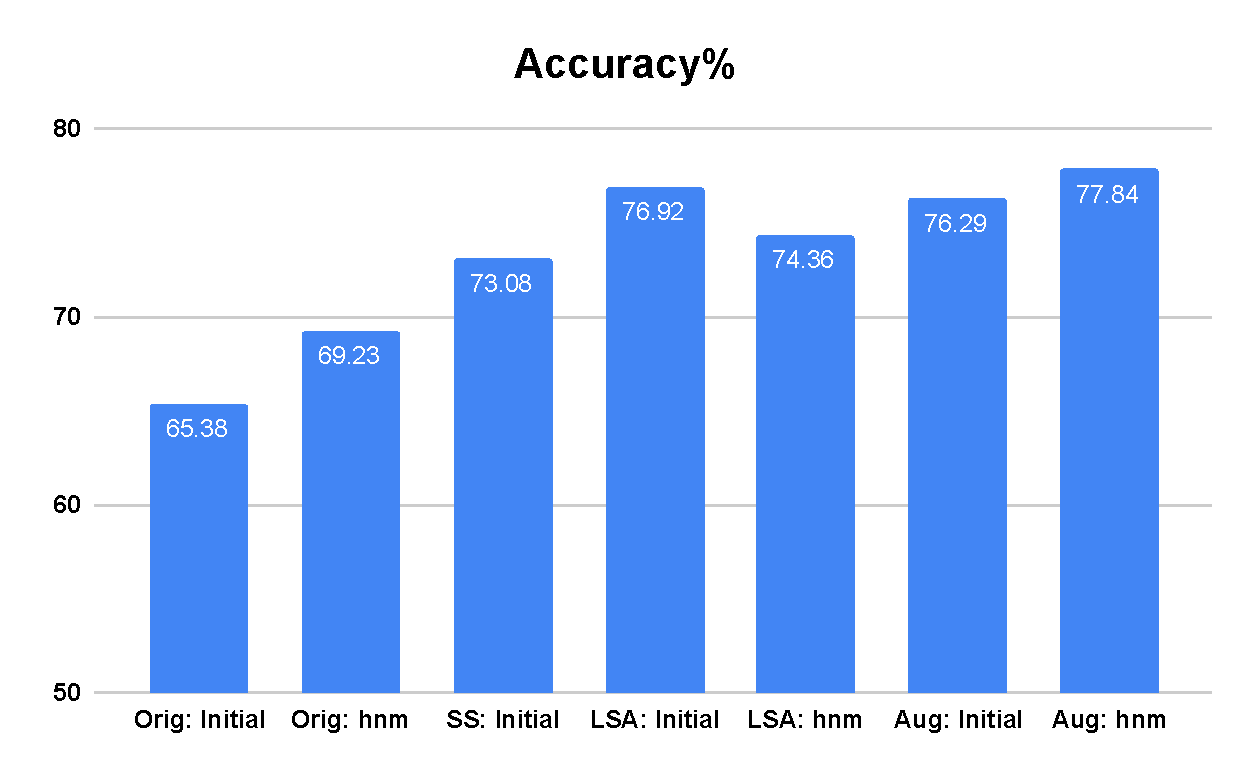
\includegraphics[scale=0.35]{Figs/chap4/baseacc.pdf}
          \caption{Accuracy}
     \end{subfigure}
     ~
     \begin{subfigure}[b]{0.5\linewidth}
         \centering
          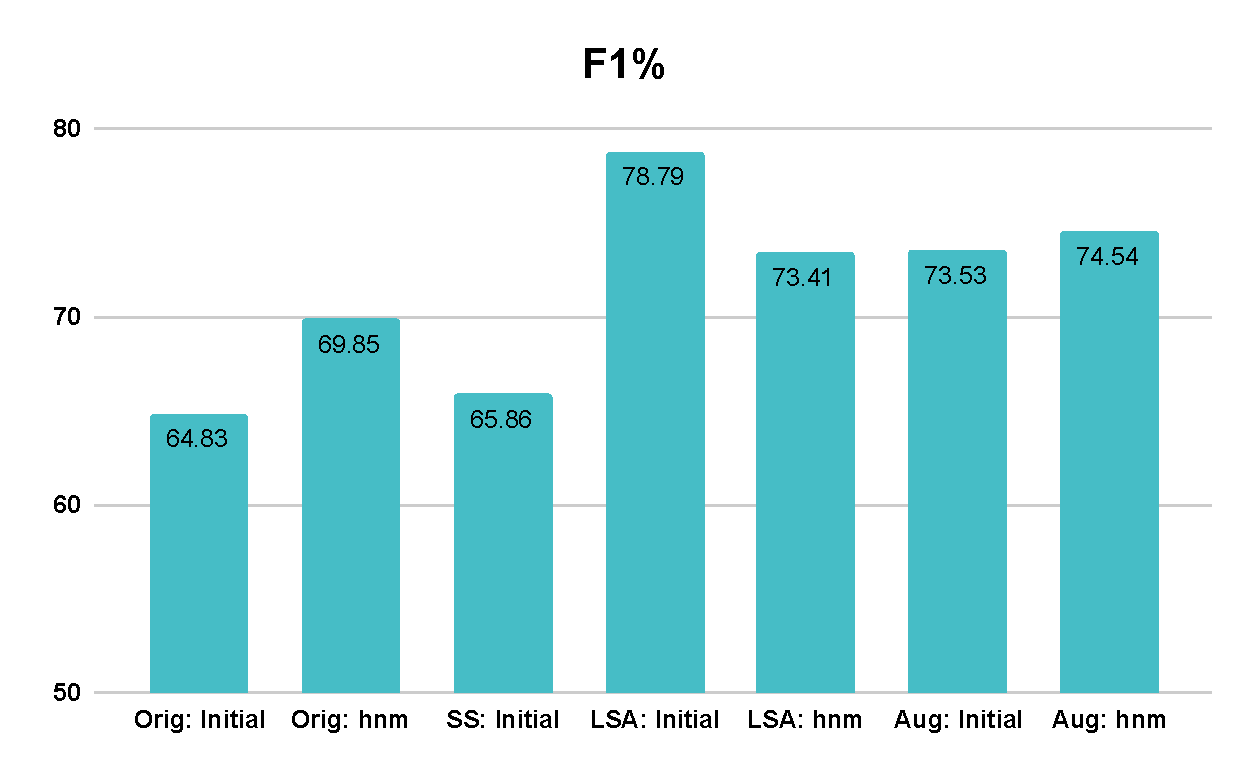
\includegraphics[scale=0.35]{Figs/chap4/basef.pdf}
          \caption{F1 score}
     \end{subfigure}
     \\
     \begin{subfigure}[b]{0.5\linewidth}
         \centering
          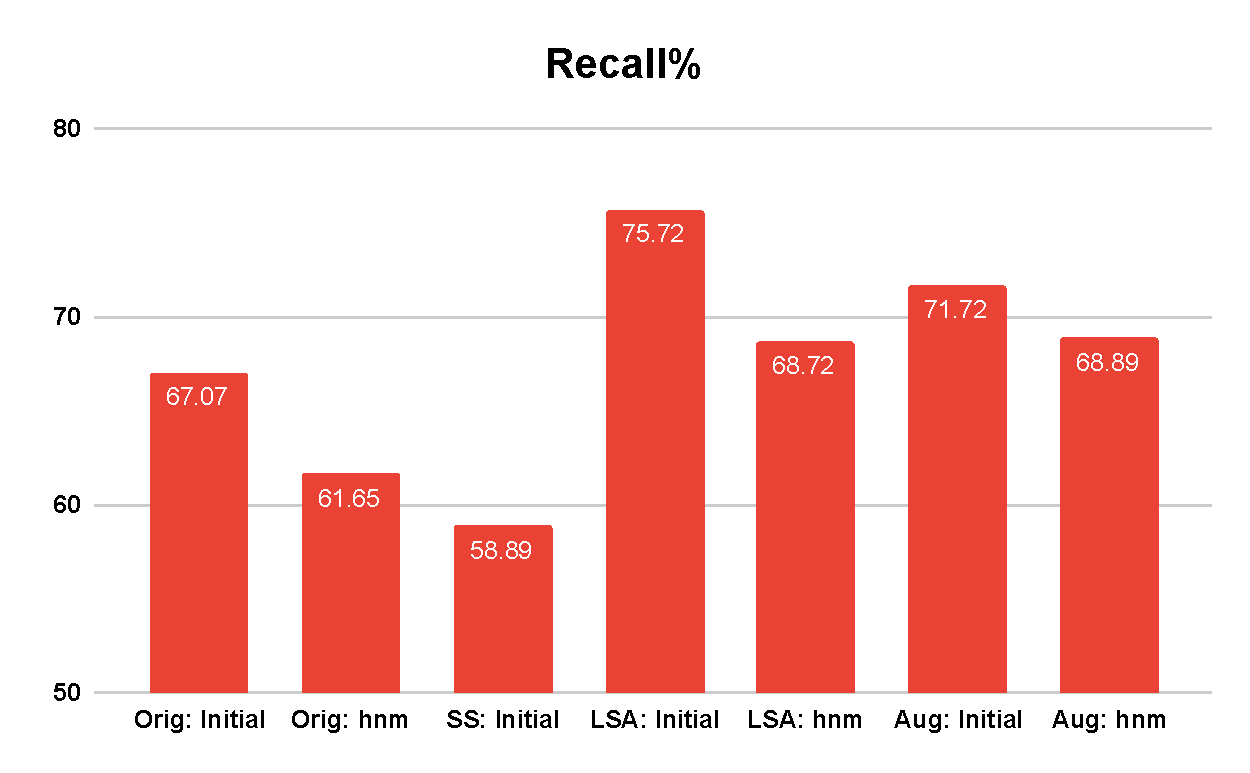
\includegraphics[scale=0.35]{Figs/chap4/baserec.pdf}
          \caption{Recall}
     \end{subfigure}
     \begin{subfigure}[b]{0.5\linewidth}
         \centering
          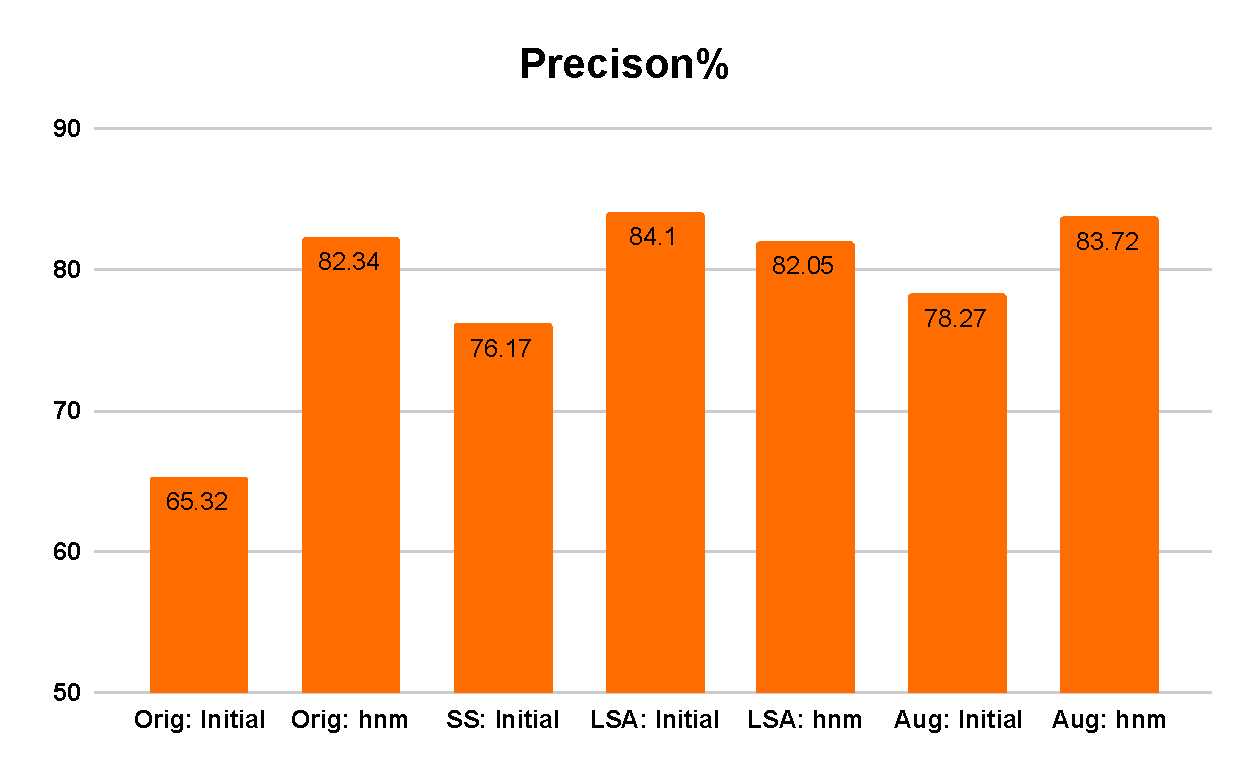
\includegraphics[scale=0.35]{Figs/chap4/basepre.pdf}
          \caption{Precision}
     \end{subfigure}
  \caption{Histograms of baseline model: comparing 7 different strategies in accuracy, F1, recall and precision}
  \label{Fig:hist}
\end{figure}
\begin{itemize}[leftmargin=*]
    \item \textbf{Original data}\\
    The results for the initial dataset without processing are same as the third column of Table \ref{tab:balanc}. After applying hard negative mining method, all metric scores are improved instead of recall. The precision significantly rises up from 65.32\% to 82.34\%, while accuracy and F1 score grow by approximate 4\%. The hard negative mining results in a reduction of recall. The possible reason is that selecting hard negatives will reduce the average distance between positives and hard negatives. Hence, the classifier can accurately recognize the hard negative with increasing precision. However, a number of hard positives (which are close to hard negatives) are affected by easy positive examples, leading to difficult classification.
    \item \textbf{Noise reduction}\\
    Since only positive calls are concerned in this project, both of spectral subtraction (SS) and MMSE-LSA denoising methods are only applied to the positive dataset before training. As shown in results, the noise reduction has the ability to improve the general performance, comparing with the dataset without processing. Specifically, the spectral subtraction retains the performance of recall to a large extent, although the accuracy and precision are improved. As introduced in Section 3.2.1, parts of the information in the region of interest were eliminated during processing, which has significantly impact on classification on positives. Thanks to its simple algorithm, SS denoising method is a time-saving process. \par
    As to MMSE-LSA approach, the results proved its effectiveness and feasibility on species detection. The model achieves impressively scores on initial dataset over whole processing strategies. Even if the accuracy is slightly lower than augmentation, the results still demonstrate its performance. However, using hard negative mining to train this model second time introduces an overall decline in performance, especial in the recall. This is same as the dataset without processing. Thus, the hard negative mining has less contribution to performance. Because we only utilized noise reduction on positive data, which affects the representation distance between positives and negatives to a large extent. Thus, hard negative seems incapable to further improve the performance. Hence, the trained model with denoised dataset may suffer from generalisation error, which is unable to provide accurate predictions on generalised tasks.
    \item \textbf{Augmentation}\\
    The model trained with the augmented dataset can reduce the generalisation error due to the variety and diversity of augmentation. The metric scores goes up over 70\% compared with the original dataset. However, the baseline model shows unremarkable results of augmentation, comparing with denoised dataset. Only accuracy of hard negative mining exceeds other strategies with 77.84\%. The baseline model is not quite deep, which can only learn relative low-level features to classify. MMSE-LSA significant remove the redundant information of mel-spectrogram. This allows the baseline model to put more attention to learn the contributive features. Although augmented dataset increases the generalisation of the model, it is still arduous for the baseline model to learn crucial features. As a result, model trained with denoised dataset obtains higher scores than augmentation. 
\end{itemize} 

In order to determine the optimal strategy for baseline model, the results are presented in visible way to compare, as shown in Fig \ref{Fig:hist}. All of the data processing methods have improved accuracy and precision with over 70\%. The accuracy has an nearly upward tendency with varying processing method. The first trained model with MMSE-LSA (LSA: Initial) and second trained model with augmentation (Aug: hnm) attain increased accuracy. The model of MMSE-LSA with initial dataset has outstanding performance on F1 and recall. However, the spectral subtraction performs underwhelming due to its recall and F1 score.
\section{VGG-based Model}
\begin{figure}[!htb]
\centering
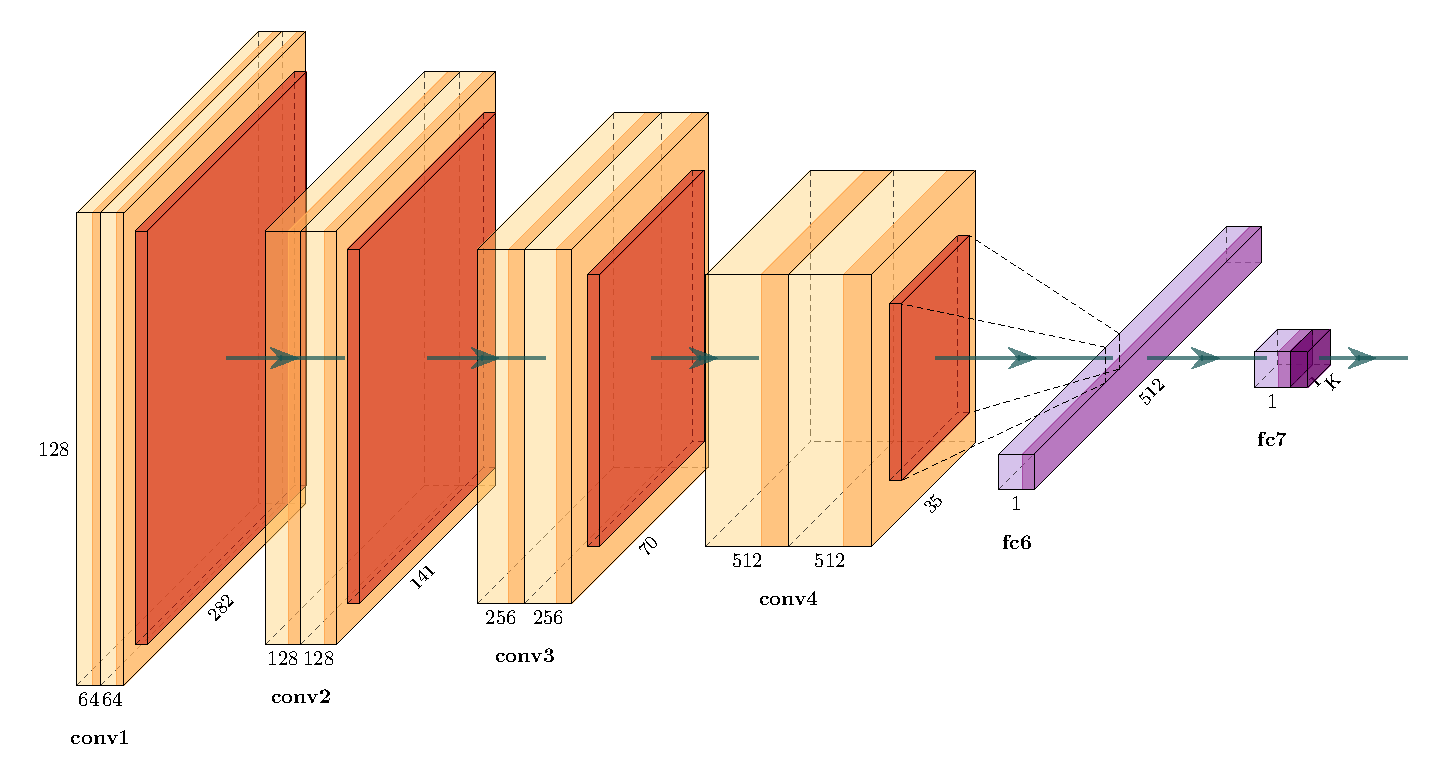
\includegraphics[scale=0.55]{Figs/chap4/vgg16.pdf}
\caption{Architecture of VGG-based CNN}
\label{fig:vgg}
\end{figure}
\subsection{Architecture}
Since the baseline model only contains three convolutional layers, low-level features were learned by this model, resulting in limited ability of detection. With the inspiration of the architecture of VGG16 \cite{simonyan2014very}, I proposed a similar network named VGG-based. Comparing with VGG16, this model is not very deep with only ten weighted layers (6 convolutional layers and 2 FC layers). The visulisation of VGG-based architecture is illustrated in Fig \ref{fig:vgg}. The $5\times5$ size filter of baseline model were replaced by two successive $3\times3$ filters, following with the maxpooling layer in size $2\times2$. For each hierarchical layers, the number of filters in convolutional layer are double, aiming to learn high-level features. Moreover, the batch normalisation layer are added after convolution. The dropout layer with ratio 0.5 was used between FC layers to prevent overfitting. Table \ref{tab:struc} compares the structure depth of baseline and VGG-based model. As a result, $4.03\times10^{7}$ parameters need to be learned, 50 times larger than baseline model. In addition, the hyperparameters for VGG-based model are same as the baseline.
\begin{table}[htp]
\centering
\caption{Comparing depth of models}
\label{tab:struc}
\resizebox{0.6\textwidth}{!}{%
\begin{tabular}{c|c|c}
\hline
 & Baseline & VGG-based \\ \hline
\multirow{3}{*}{1} & conv(24,5,5) & conv(64,3,3) \\
 &  & conv(64,3,3) \\
 & maxpooling(4,2) & maxpooling(2,2) \\ \hline
\multirow{3}{*}{2} & conv(48,5,5) & conv(128,3,3) \\
 &  & conv(128,3,3) \\
 & maxpooling(4,2) & maxpooling(2,2) \\ \hline
\multirow{3}{*}{3} & conv(48,5,5) & conv(256,3,3) \\
 &  & conv(256,3,3) \\
 &  & maxpooling(2,2) \\ \hline
\multirow{3}{*}{4} &  & conv(512,3,3) \\
 &  & conv(512,3,3) \\
 &  & maxpooling(2,2) \\ \hline
\multirow{2}{*}{FC} & FC128 & FC512 \\
 & FC1 & FC1 \\ \hline
 & \multicolumn{2}{c}{sigmoid} \\ \hline
\#param & $8.61\times10^{5}$ & $403\times10^{5}$ \\ \hline
\end{tabular}%
}
\end{table}
\subsection{Results}
\begin{table}[htp]
\centering
\caption{Metrics score of Complex VGG-like model with three dataset strategies}
\label{tabel:VGG dataset}
\resizebox{0.9\textwidth}{!} & \textbf{Precision\%}  & \textbf{Recall\%}& \textbf{F1 score\%}\\
\hline
\textbf{Orig: Initial}& 71.79 & 71.45 & 73.54 & 72.05 \\
\textbf{Orig: hnm} & 70.51 & 75.28 &  76.13 & 75.13\\ 
\hline
\textbf{LSA: Initial} & 76.92 & 81.72 &  77.96 & 79.64\\ 
\textbf{LSA: hnm}& 73.08 & 72.96 &  73.84 & 73.22\\
\hline
\textbf{Aug: Initial}  & 84.54 & 84.59 & \textbf{85.94} & \textbf{84.27}\\
\textbf{Aug: hnm}& \textbf{85.05} & \textbf{89.74} &79.56 & 83.32\\ 
\hline
\end{tabular}}
\end{table}
The VGG-based model was trained in the same way as discussed in baseline model. Due to the increased depth, the VGG-based model effectively improved the performance. Table \ref{tabel:VGG dataset} illustrated the metric scores of these methods. Note that the spectral subtraction did not test in VGG-based model since its underwhelming performance. Training VGG-based model took more than 10-fold time on CPU. Thus, all training works were completed on Amazon Web Services (AWS) by GPUs, with approximate 15 minutes on small dataset and 50 minutes on augmentation. 
\begin{itemize}[leftmargin=*]
    \item \textbf{Original data}\\
     By learning high-level features, the VGG-based model with initial dataset without processing can attain scores over 70\%. After applying hard negative mining, the performance is further improved by approximate 3\% in precision, recall and F1 score. Comparing with the same dataset of baseline model, only precision has impressive scores in 82.34\%. Nevertheless, the training work for VGG-based model is significant time-cost than baseline model.
    \item \textbf{Noise reduction}\\
    The noise reduction method provides less contributive improvement of VGG-based model. Metric scores are approximately similar to the baseline of denoising dataset. Because the MMSE-LSA removed most of the background noise, high-level features can not be further learned by increasing depth of architecture. Additionally, applying hard negative mining on denoised data causes a decreasing performance on VGG-based model as well. It indicates that training with denoised dataset will introduce bias for classification. The model only can detect the positive call without noise, leading to limited robust on noise.
    \item \textbf{Augmentation}\\
    Training with augmentation dataset achieves prominent results for VGG-based model. All scores reach or exceed 80\%, presenting in enhanced accuracy and precision about 85.05\% and 89.74\%with hnm dataset. Nevertheless, the hard negative mining still introduces a decline in recall about 6\%, resulting in relatively decreased F1 score. With contributions of augmentation, the VGG-based model can learn various and diverse data in high-level representation. On the contrary, the shallow network is incapable to effectively classified with low-level features, even if data were augmented in increased variety and diversity.
\end{itemize}
As illustrated in Fig \ref{Fig:histvgg}, the VGG-based model after augmentation significantly outperforms noise reduction. The denoised dataset with using hnm has relatively low performance. It is caused by that MMSE-LSA is not a lossless technique, which may introduce attenuation and disturbance on audio data. After using hard negatives, the distance is more indistinguishable between positives and negatives. In total, training with augmentation dataset and hnm results in an optimal VGG-based model.
\begin{figure}[!htb]
     \begin{subfigure}[b]{0.5\linewidth}
         \centering
          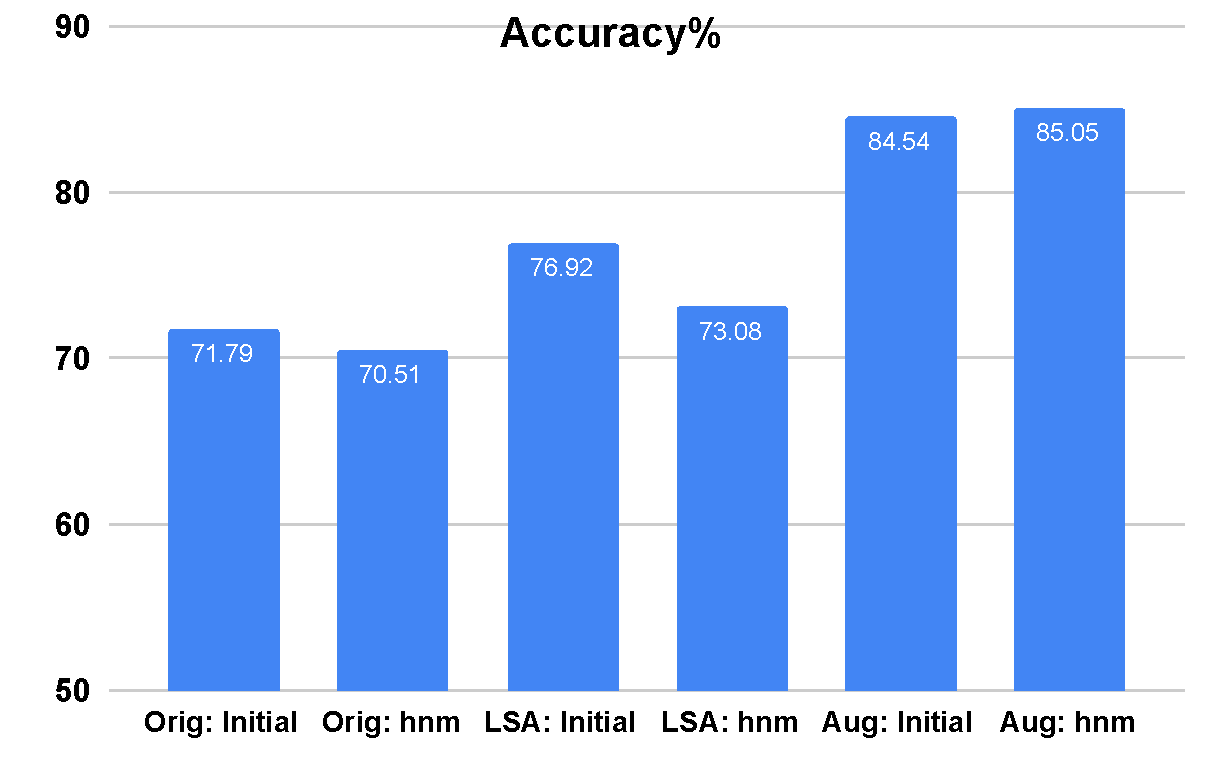
\includegraphics[scale=0.35]{Figs/chap4/vggacc.pdf}
          \caption{Accuracy}
     \end{subfigure}
     ~
     \begin{subfigure}[b]{0.5\linewidth}
         \centering
          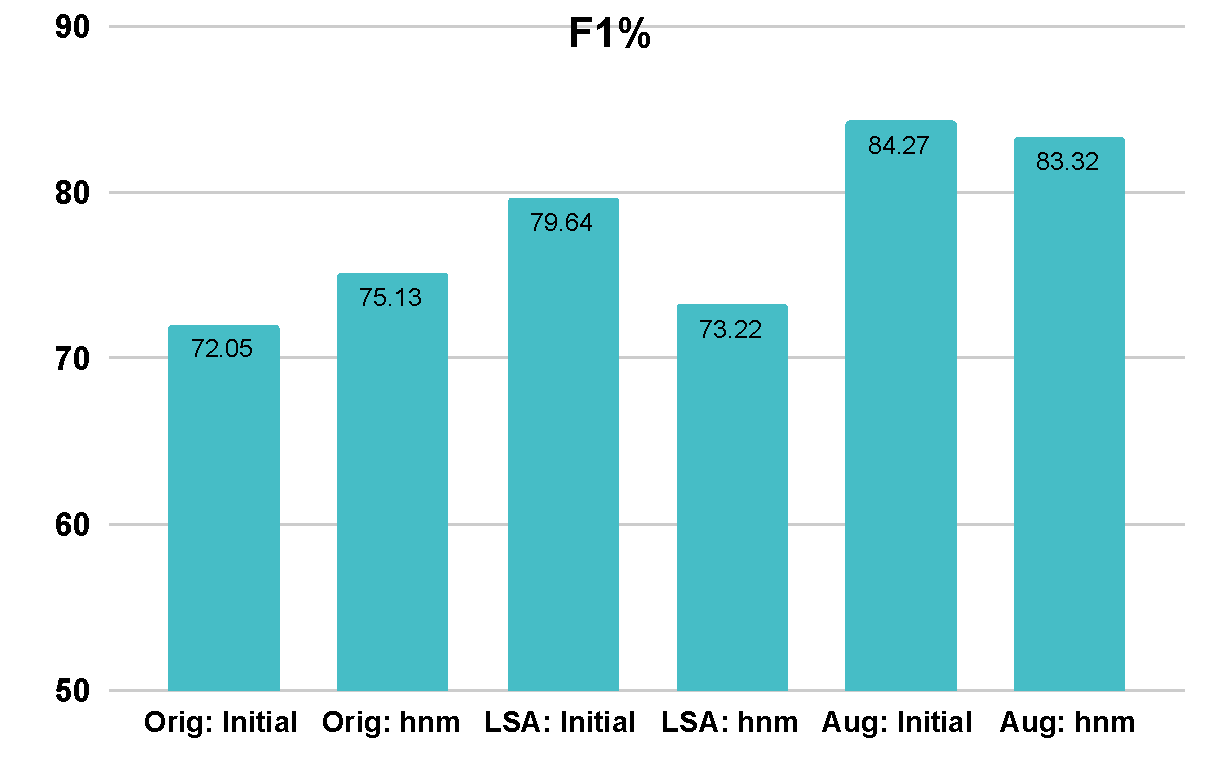
\includegraphics[scale=0.35]{Figs/chap4/vggf.pdf}
          \caption{F1 score}
     \end{subfigure}
     \\
     \begin{subfigure}[b]{0.5\linewidth}
         \centering
          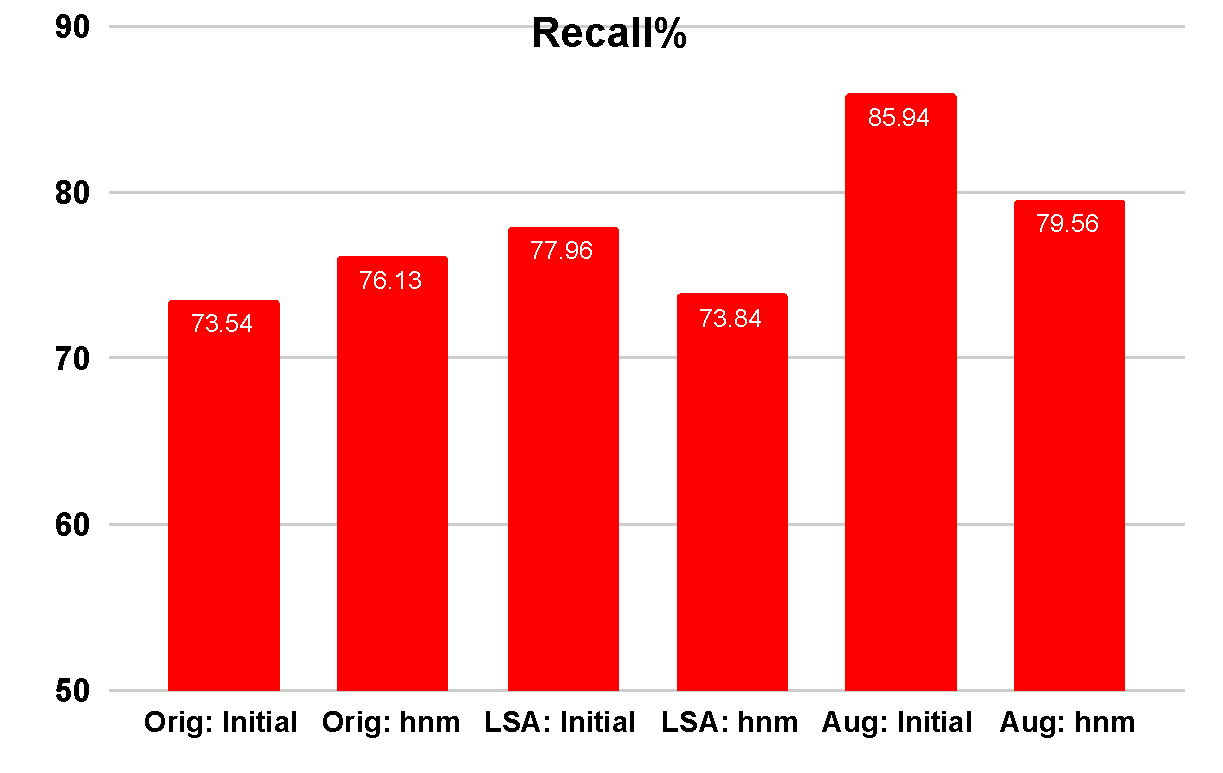
\includegraphics[scale=0.35]{Figs/chap4/vggrec.pdf}
          \caption{Recall}
     \end{subfigure}
     \begin{subfigure}[b]{0.5\linewidth}
         \centering
          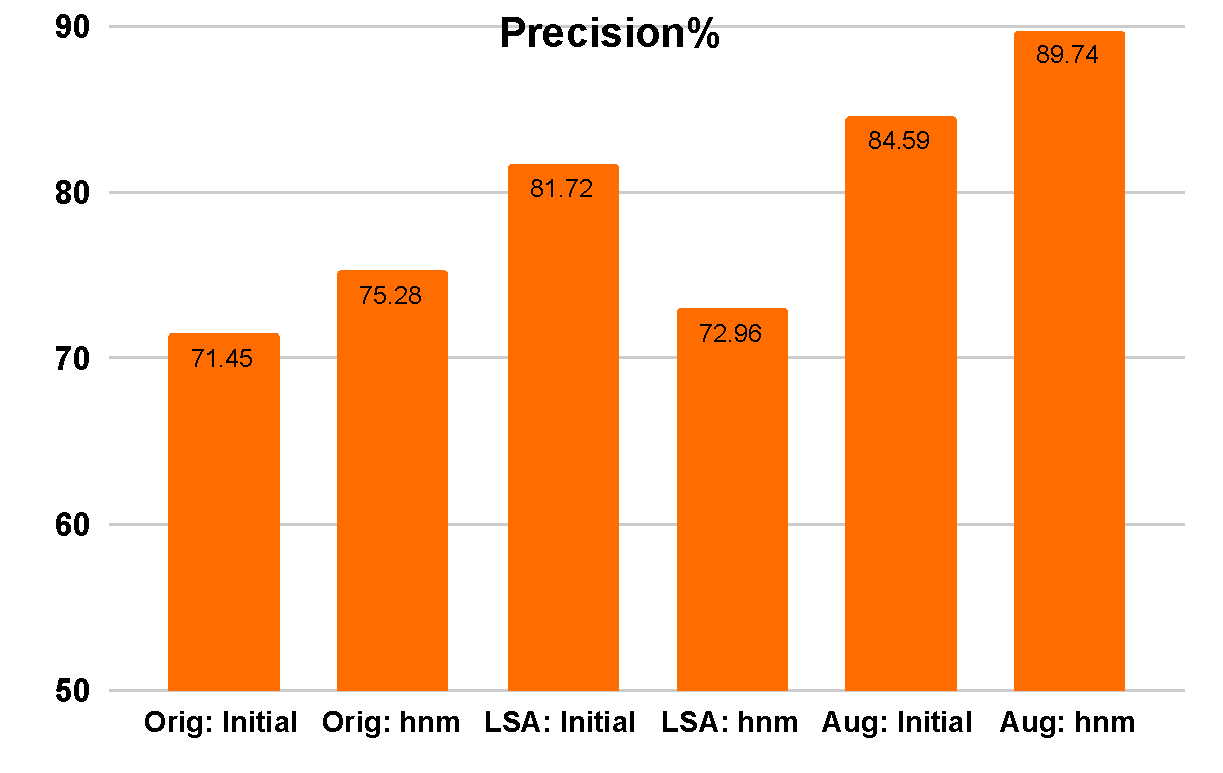
\includegraphics[scale=0.35]{Figs/chap4/vggpre.pdf}
          \caption{Precision}
     \end{subfigure}
  \caption{Histograms of VGG-based model: comparing 7 different strategies in accuracy, F1, recall and precision}
  \label{Fig:histvgg}
\end{figure}
\subsection{Position Detection on New Testing Data}
As illustrated previously, the metric scores were measured on fix dataset to evaluate the model performance. In order to compare the capability of generalisation among models, new test data were manipulated to examine the predictions of trained models. All audio files were clipped into 3-seconds segments, resulting in totally 4660 clips. Each clip records its clipped position in the raw audio file. Afterwards, the trained models are used to predict all clips and compare the actual position label in 'Praat' files. The prediction is considered as false positive if it not only was incorrectly classified but also has over 90\% confidence scores (the output of sigmoid in the last layer of network presenting in percentage). Table \ref{tab:wrong pos} shows the number of wrong predictions for trained models of all strategies. The less wrong predictions were detected, the higher capability of generalisation.\par
\begin{table}[htp]
    \centering
    \caption{Wrong predicted positions of two models}
    \label{tab:wrong pos}
    \resizebox{0.8\textwidth}{!}{%
    \begin{tabular}{|l|cc|cc|}
    \hline
     & \multicolumn{2}{c|}{Baseline} & \multicolumn{2}{c|}{VGG-based} \\ \cline{2-5} 
     & \multicolumn{1}{c|}{Num.} & Error\% & \multicolumn{1}{c|}{Num.} & Error\% \\ \hline
    Orig: Initial & 876 & 18.79 & 517 & 11.09 \\
    Orig: hnm & 748 & 16.05 & 421 & 9.03 \\ \hline
    LSA: Initial & 479 & 10.27 & 309 & 6.63 \\
    LSA: hnm & 455 & 9.76 & 280 & 6.01 \\ \hline
    Aug: Initial & 389 & 8.35 & 203 & 4.36 \\
    Aug: hnm & \textbf{353} &\textbf{7.58} & \textbf{157} & \textbf{3.37} \\ \hline
    \# average time (mins) & \multicolumn{2}{c|}{3.74} & \multicolumn{2}{c|}{32.36} \\ \hline
    \end{tabular}%
    }
\end{table}
In general, the incorrect number of prediction is descending with the order of strategies for both models. Using hard negatives to train model second time can optimize model to a certain extent. As to baseline, the MMSE-LSA shows outstanding scores with 84.41\% accuracy and 78.79\% F1 score in Table \ref{tabel:base dataset}, based on which this model was optimal. However, the number of wrong position for augmentation dataset is minimum, which means the generalisation error is lower than denoised dataset. There are two main reasons caused the higher generalisation error of denoised dataset. Firstly, the number of denoised training data is quite smaller than the augmentation, which is not enough to completely train the network. Furthermore, it will introduce classification bias only trained model with denoised positives. Sine pure speech signals are unavailable in most of realistic situations, this trained model has limited ability to detect positive calls. However, denoising is still helpful to classify negative examples.

As to VGG-based model, results demonstrate that it has powerful and effective performance on classification, with 3.37\% error for augmentation. Therefore, increasing the architecture depth of network can significantly enhance the ability of robustness and generalisation. Nevertheless, the main drawback for VGG-based model is time. Due to the increasing number of parameters and depth of network, both training and predicting are time-consuming efforts, compared with baseline model. It took 8.33 seconds on average for VGG-based model to predict one-minute long file, while baseline took less than 1 second.
However, it is still prominently efficient and effective than manually labelling. Although there were still amounts of wrong positions, all prediction results were recoded in file, which is beneficial to further manual check.
\section{Comparison of Optimal Models}
\begin{figure}[!htb]
     \begin{subfigure}[b]{0.5\linewidth}
         \centering
          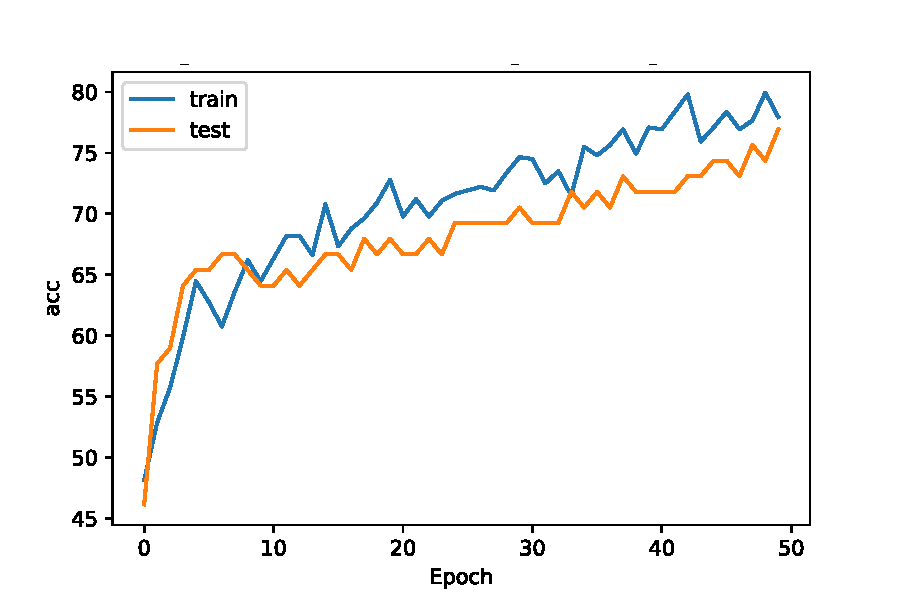
\includegraphics[scale=0.5]{Figs/chap4/denoised_e50_b16_acc.pdf}
          \caption{Baseline: accuracy }
     \end{subfigure}
     ~
     \begin{subfigure}[b]{0.5\linewidth}
         \centering
          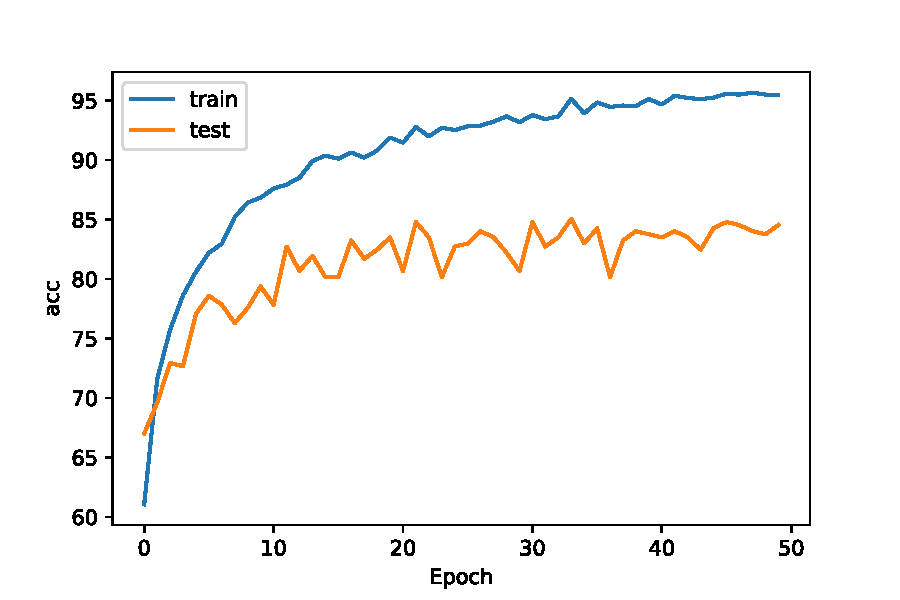
\includegraphics[scale=0.5]{Figs/chap4/vgg_augment_denoise_e50_b16_acc.pdf}
          \caption{VGG-based: accuracy }
     \end{subfigure}
     \\
     \vskip0.5em
     \begin{subfigure}[b]{0.5\linewidth}
         \centering
          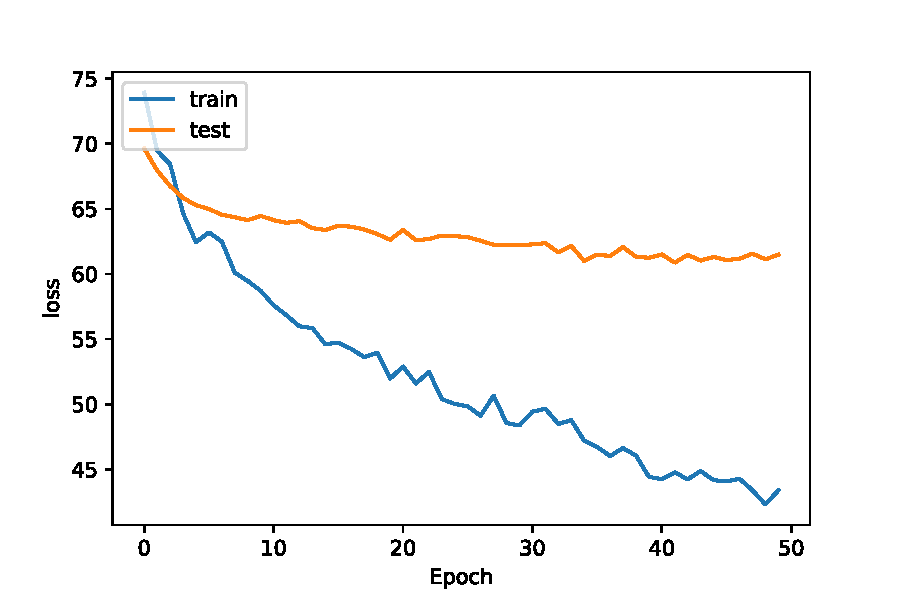
\includegraphics[scale=0.5]{Figs/chap4/denoised_e50_b16_loss.pdf}
          \caption{Baseline: loss}
     \end{subfigure}
     \begin{subfigure}[b]{0.5\linewidth}
         \centering
          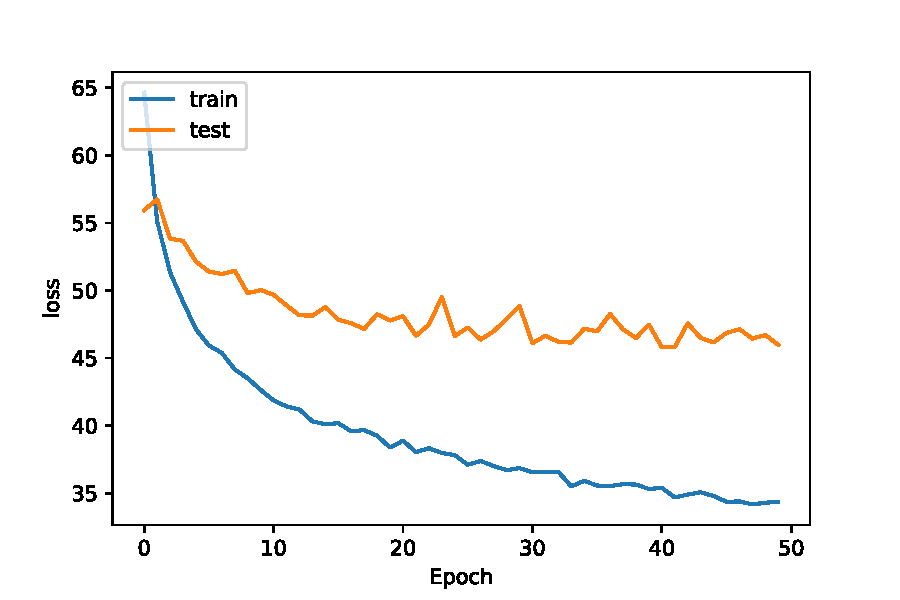
\includegraphics[scale=0.5]{Figs/chap4/vgg_augment_denoise_e50_b16_loss.pdf}
          \caption{VGG-based: loss}
     \end{subfigure}
  \caption{Accuracy and loss curves for optimal baseline (LSA: Initial) and VGG-based models (Aug: hnm) with epoch=50, batch\_size=16, lr=$10^{-5}$}
  \label{Fig:curve}
\end{figure}
Fig \ref{Fig:curve} depicts the accuracy and loss curves of two optimal model. The train and test accuracy have less difference for baseline model. Both of them gradually rise up and reach peak point with approximate 75\%. As to the VGG-based model, the training accuracy rapidly increases to 90\% at 15 epochs. Afterwards, both of accuracy curves gently increase until convergence. As a consequence, the test accuracy reaches 85.5\%, while the accuracy of training is up to 95\%. The test loss of denoised dataset for baseline model is difficult to reduce compared with VGG-based model. Thus, the gap between test and train loss is getting larger with increasing epochs. This may bring out the over-fitting problem with high generalisation error. However, the VGG-based model is significant robust and steady. The test loss can converge to approximately 0.45 after 50 epochs. Overall, the VGG-based architecture can effectively improve the classification performance, with relative outstanding metric scores and generalisation error.\par

Observing scores in Table \ref{tabel:base dataset} and Fig \ref{Fig:hist}, recall is generally lower than accuracy among all strategies. It means that certain positives are always classified as false negatives by baseline model, which indicates that there are a number of hard positive in the training dataset. Fig \ref{Fig:type} illustrates four types of positive and negative with easy and hard examples respectively. By comparing the difference of mel-spectrogram among examples, reasons for limited performance on positive data can be found. \par
\begin{figure}[!htb]
\hspace*{-2em}
     \begin{subfigure}[b]{0.5\textwidth}
         \centering
          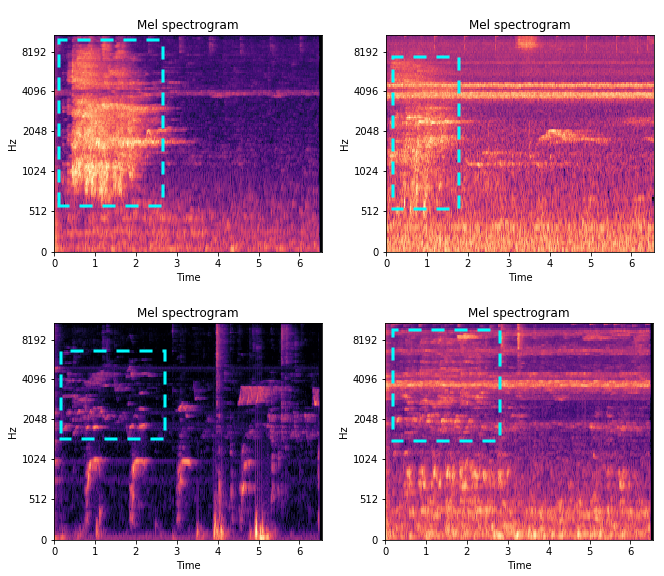
\includegraphics[scale=0.33]{Figs/chap4/pos.png}
          \caption{\centering Positive calls: Clear call (top\_left); Clear$+$Noise (top\_right); Unclear call (low\_left); Unclear$+$Noise (low\_right)}
     \end{subfigure}
     \hfill
     \begin{subfigure}[b]{0.5\textwidth}
         \centering
          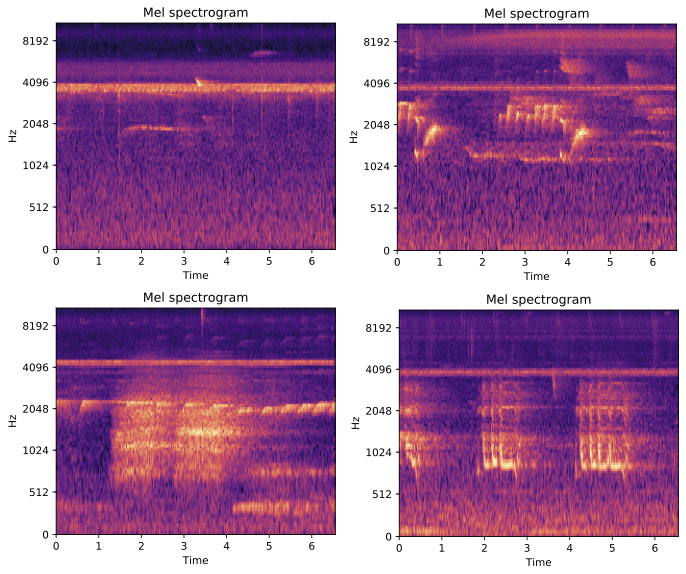
\includegraphics[scale=0.33]{Figs/chap4/neg.png}
          \caption{\centering Negative: Environmental noise (top\_left); Bird (top\_right); Howler monkey (low\_left); Macaws (low\_right)}
     \end{subfigure}
  \caption{Types of positives and negatives with easy and hard examples}
  \label{Fig:type}
\end{figure}
The quality of positives is relatively inconsistent during data collection. There are approximately four types of positives, namely clear calls (easy positives); clear calls covered by noise (relatively easy); unclear calls (relatively hard); unclear calls covered by noise (hardest). As to negatives, the environmental noise is the easy negative sample, while other animal calls (bird, Howler monkey and macaws et al.) increase difficulties on classification. Howler monkey calls have similar spectral characteristics in frequency and time. This similarity between negative spectrograms and hard positives confused the baseline model to a large extent. Hence, it is an arduous task for baseline to detect hard positives using low-level features, leading to lower recall than accuracy. After applying hard negative mining method, the distance of centres between negatives and positives tends to shrink, resulting in increased precision and decreased recall. Thus, hard positive mining can be applied as a further improvement. However, the VGG-based model slightly suffers from this issue, since high-level features can be extracted even from unclear calls. 



% !TEX root=../main.tex
\chapter{Conclusion}
\renewcommand{\baselinestretch}{\mystretch}
\label{chap:Conclusion}
%\setlength{\parindent}{0pt}
\PARstart{T}{his} report proposed an automated audio detector based on the CNN architecture. The architecture of shallow network was implemented as baseline model. Mel-spectrogram is beneficial to represent audio signals due to its perceptual features.
It has been demonstrated that normalisation and balancing are essential before training, especially in data with large within-class variance. Moreover, we have investigated the improvement of several data processing methods. Performances of two noise reduction methods, namely spectral subtraction (SS) and MMSE-LSA estimators, were compared with visualisations of mel-spectrogram and model scores. The model with initial dataset using MMSE-LSA achieved outstanding scores in accuracy 84.1\% and F1 score of 78.9\%. However, the denoising method blurred the region of interest to some extent, leading to a relative higher generalisation error. The augmentation approach increased the variety and diversity of dataset, resulting in a decreased generalisation error. 

In order to further improve the performance, an deep neural network was proposed with the inspiration of VGGNet. The performance was limited for the baseline model due to the shallow architecture. Increasing network depth prominently improved the performance on classification. With the contributions of high-level features, the VGG-based model has the ability to learn hard positive examples. The optimal VGG-based model with augmentation data achieved expressively scores of accuracy in 85.05\% and F1 score in 83.32\%.  Even though training and predicting are time-cost work for VGG-based model, it is still significantly effective and efficient compared with manually labelling. Furthermore, hard negative mining was applied to train models a second time, which improve the accuracy and precision. Although there were a number of wrong predicted positions for all models, the prediction record was created in files for further manually check.

% !TEX root=../main.tex
\chapter{Future Works}
\renewcommand{\baselinestretch}{\mystretch}
\label{chap:Future}
%\setlength{\parindent}{0pt}''
\PARstart{D}{ue} to the limitation of time, some improvements can be further applied to this project. The essential way of reducing the model mineralisation error is to use more data to train the model. In the future, more audio data with high-quality calls could be added to the training set. In this project, all of 128 mel frequency features are extracted as the representations of input. If the spectral characteristics of spider monkey can be investigated firstly, we can reduce the number of coefficients and focus on the specific frequency region. The spectrogram after modifying will decrease the input shape of CNN, leading to faster computation. Other state-of-art CNN architectures could be applied as well, since the time of perdition for VGG-based model is a bit slow.

Hard negative mining was used to train the model second time, resulting in increasing precision but decreasing recall. The hard positive mining could be utilized as well to make model learn the undistinguishable positive feature. Since the denoising approaches will affect the informative region of spectrogram to some extent. A developed strategy can be suggested that only perform noise reduction method for the signal with lower SNR. This would introduce an extra work to estimate the signal SNR at first.

As studied in \cite{hermans2017defense}, triplet loss
shows better performance than hard negative mining on person re-identification problem. I have tried to construct triplets with anchor, positive and negative samples. Afterwards, train the model to learn embeddings and use the nearest neighbour to classify. However, due to the binary classification problem and lack of training data, results show worse performance than binary cross-entropy. The reason could be further investigated.

As to data augmentation method, Google AI \cite{park2019specaugment} has proposed to perform data augmentation directly on spectrogram, named SpecAugment. They applied several masks to block the information on the spectrogram with randomly determined size. The vertical mask blocks the consecutive time information and the horizontal mask is for frequency channels. Experiments have demonstrated its better performance on automatic speech recognition. Thus, it can be an alternative augmentation on species detection.




\renewcommand{\baselinestretch}{1}

% Note: put the bib style and bib file you use here.
\bibliographystyle{IEEEtran}
\bibliography{references}
\fancyhead[RE]{\emph{References}}
\appendix
% !TEX root=../main.tex

\renewcommand{\baselinestretch}{1.5}
\chapter{Baseline CNN Model}
\begin{figure}[htbp]
     \begin{subfigure}[b]{0.5\linewidth}
         \centering
		  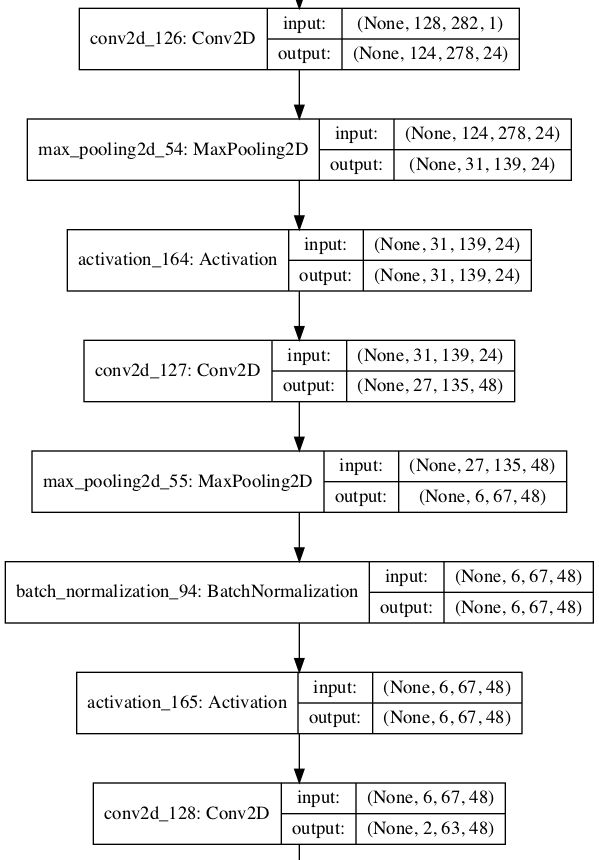
\includegraphics[scale=0.35]{Figs/Appen/simple_model_plot.png}
     \end{subfigure}
     ~
     \begin{subfigure}[b]{0.5\linewidth}
         \centering
		  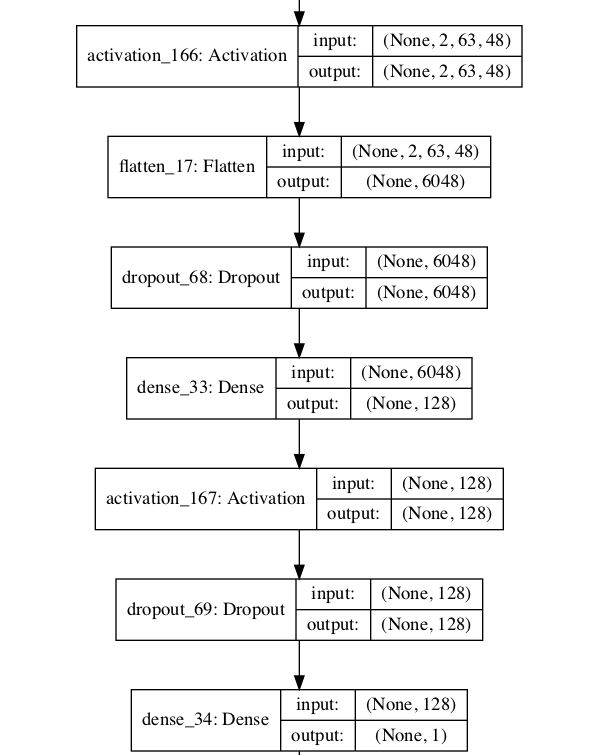
\includegraphics[scale=0.35]{Figs/Appen/simple_model_plot2.png}
     \end{subfigure}
  \caption{Structure of baseline model}
  \label{Fig:shapebaseline}
\end{figure}
\chapter{VGG-based CNN Model}
\begin{figure}[htbp]
      \centering
      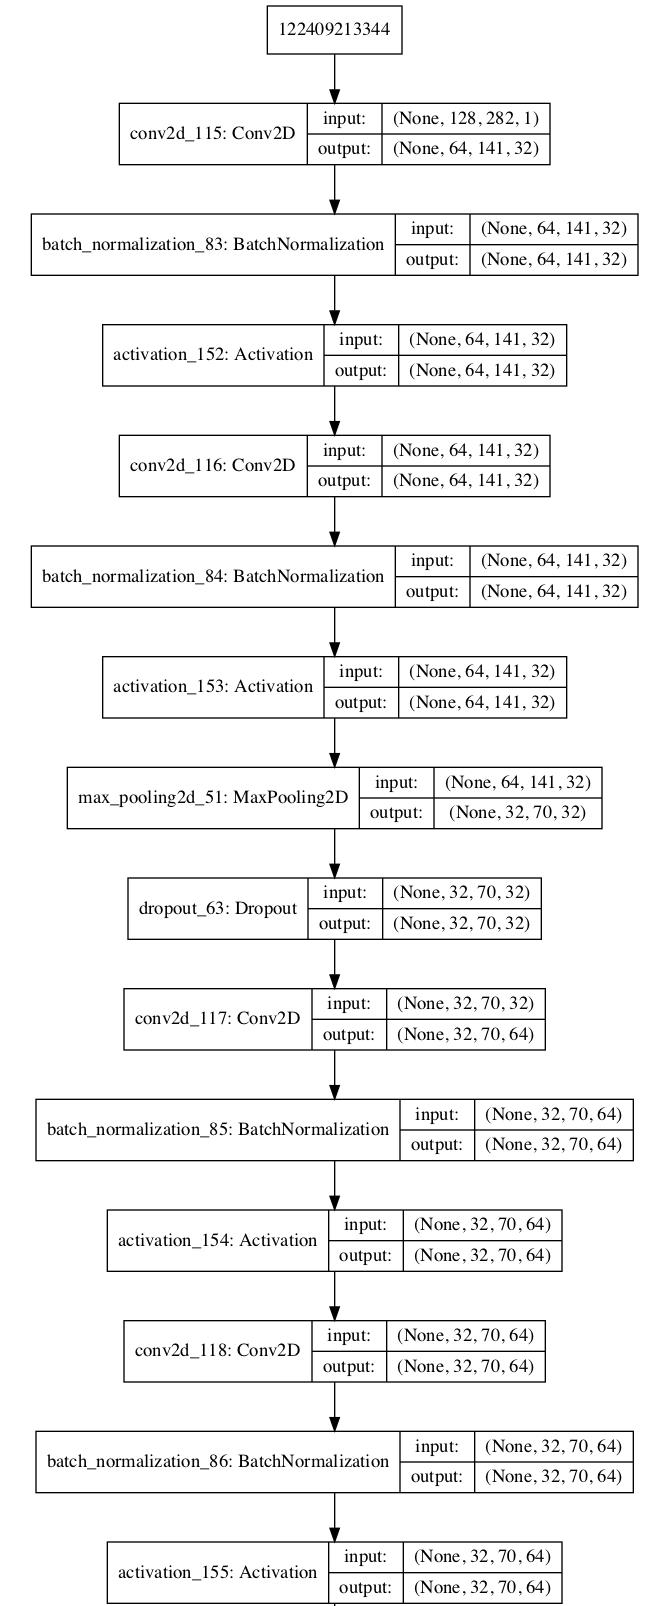
\includegraphics[scale=0.35]{Figs/Appen/model_plot1.png}
\end{figure}
\begin{figure}[htbp]
\centering
     \begin{subfigure}[b]{0.45\linewidth}
      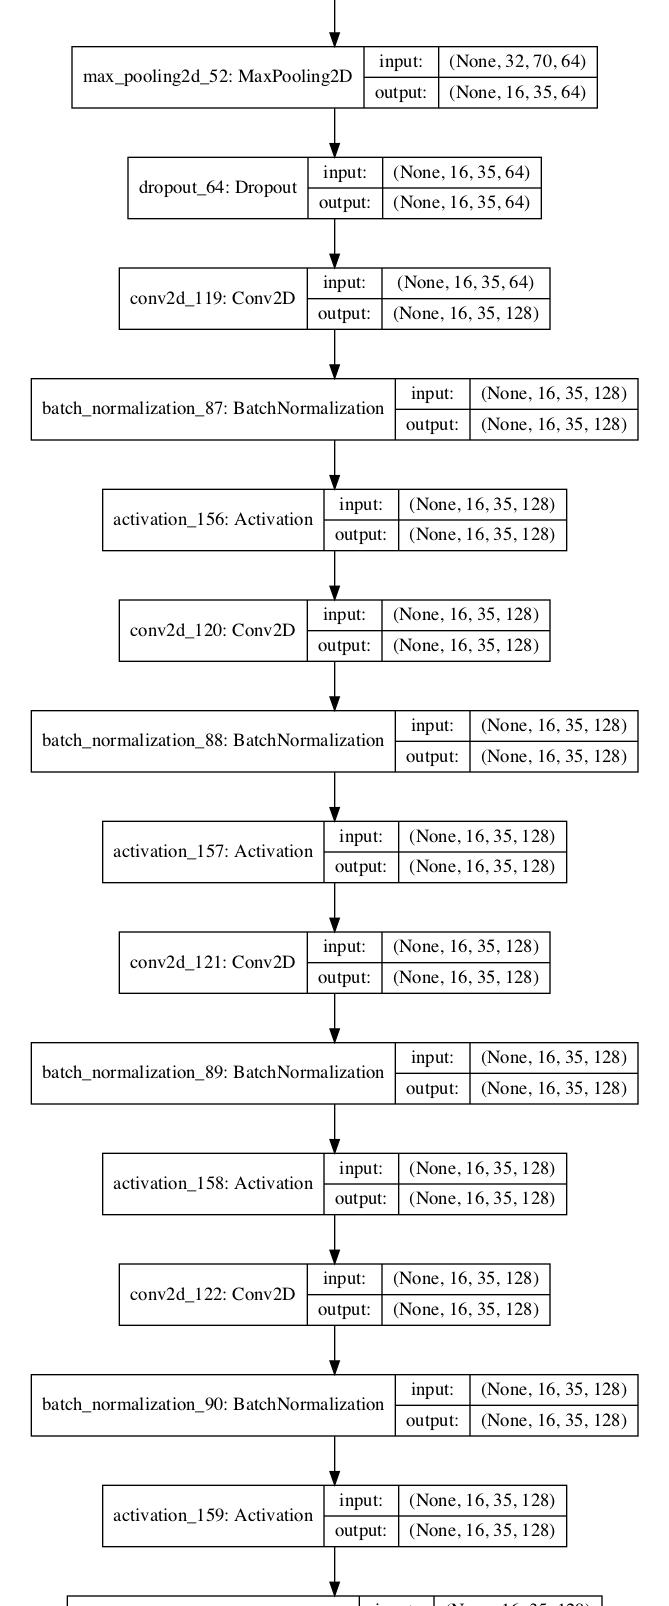
\includegraphics[scale=0.35]{Figs/Appen/model_plot2.png}
     \end{subfigure}
          \begin{subfigure}[b]{0.45\linewidth}
      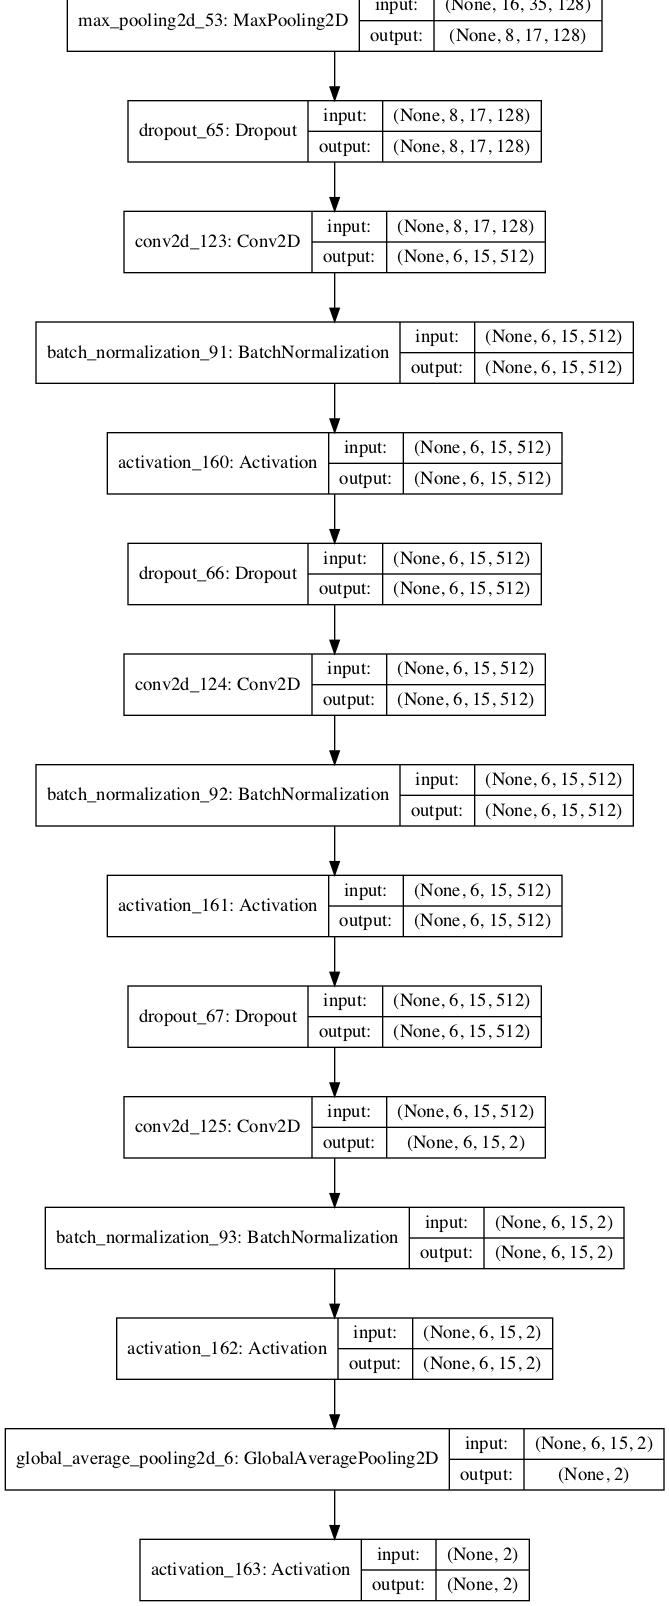
\includegraphics[scale=0.35]{Figs/Appen/model_plot3.png}
     \end{subfigure}
  \caption{Structure of VGG-based model}
  \label{Fig:shapevgg}
\end{figure}
%%%%%%%%%%%%%%%%%%%%%%%%%%%%%%
% The end of a LaTeX document
\end{document}

%%%%%%%%%%The END%%%%%%%%%%%%%%%%%%%% 